
\chapter{Image-Based Visual Servo Docking Control}

Autonomous aerial refueling (AAR) can effectively increase the combat range of aircraft, which is crucial to the future development of long-endurance aircraft. However, AAR has a high accident rate, and it has become increasingly urgent to design efficient and safe methods or algorithms for solving AAR problems. The probe-and-drogue refueling (PDR) system is considered simpler, lighter, and more easy-to-install than other aerial refueling systems. However, the docking difficulty of PDR is high. Apart from the various aerodynamic disturbances, another problem is the pose estimation error caused by the camera installation error, calibration error, and/or 3D object modeling error, which may violate the highly accurate docking requirement. This paper aims to implement an image-based visual servo control method for the AAR docking control problem. The corresponding image-based visual servo controller is designed after the establishment of an image-based visual servo model involving the receiver's dynamics. Simulation results indicate that the proposed method can make the system dock successfully under complicated environments and meanwhile improve the robustness against pose estimation error.

\section{INTRODUCTION}
Autonomous aerial refueling (AAR) can effectively increase the combat range of unmanned aerial vehicles (UAVs), which is crucial to the future development of long-endurance aircraft. \cite{nalepka2005automated}. The probe-and-drogue refueling (PDR) system is considered simpler, lighter, and more easy-to-install than other aerial refueling systems. However, the control problem of PDR is more complicated than other aerial refueling methods. The drogue is susceptible to aerodynamic disturbances in PDR because of the flexibility of the hose-drogue assembly \cite{THOMAS201414,DAI2016448,7738351}. Moreover, PDR calls for high-precision  requirements of the relative `tanker-receiver' or `drogue-probe' position and orientation during the docking stage. Therefore, it is challenging to design a reliable and robust docking controller for the receiver aircraft. 

Various sensing technologies have been employed in PDR, including the global positioning system (GPS), inertial navigation systems, electro-optical systems, etc. \cite{THOMAS201414,martinez2013vision}. Although these sensors can be adopted for autonomous aerial docking, they all have limitations in practice. For instance, the receiver's GPS signals might be unavailable when shadowed or distorted by the tanker. In recent years, machine vision technologies have been proposed to complement these technologies \cite{parry2023review}. Some vision-based navigation systems can be found in Refs. \cite{martinez2013vision,valasek2005vision,wang2015real}. Ref. \cite{campa2004autonomous} combined the GPS navigation system with vision systems.  Ref. \cite{sun2019bionic} adopted GPS navigation when the probe is far from the drogue and adopted bionic visual navigation for close-range situations. 


With the development of visual navigation systems, visual servo control has become increasingly popular in AAR. The existing visual servo control schemes are classified as position-based visual servos (PBVS) and image-based visual servos (IBVS). The main difference between PBVS and IBVS is how the features are designed.  
In PBVS, the features are 3D parameters, for example, the pose of the camera relative to some coordinate frames, which must be calculated from image information \cite{chaumette2006visual,chaumette2007visual,campa2009simulation}. The most commonly-used method is to deploy marks on the parachute part of a drogue by using infrared light emitting diodes (LEDs) \cite{wang2015real}, and then use the Gaussian least-square-differential-correction (GLSDC) algorithm \cite{valasek2005vision} or a deep learning method \cite{choi2021study,liu2018deep} to obtain relative pose. 
In IBVS, the features consist of 2D features that are immediately available from the image information \cite{chaumette2006visual}. 
The visual servo control method has been applied to AAR systems by many researchers \cite{sun2019bionic,tandale2006trajectory,duan2020bionic,valasek2017fault}. Ref. \cite{duan2020bionic} designed a docking controller based on sliding mode control and backstepping design after precise pose estimation by visual navigation methods. Moreover, control methods like iterative learning control \cite{dai2018terminal,ren2019reliable} and fault-tolerant control \cite{valasek2017fault} have also received much attention. These studies mainly focus on pose estimation methods and corresponding controller design to provide the relative ?tanker-receiver? and ?drogue-probe? position and achieve a robust and safe approach and docking. 


On the whole, there still exist some challenges in visual servo control for PDR. First, the system model of the PDR docking is complicated. The hose is flexible, and whose motion is easily affected by disturbances. Besides, there are complex disturbances during the docking process. For example, the bow wave disturbance around the receiver nose is state-dependent and nonlinear \cite{DAI2016448,7738351}. Moreover, it should be noted that a high-precision 2D image observation does not imply a high-precision pose estimation due to the camera installation error, calibration error, and/or 3D object modeling error \cite{garcia2021real}. Existing works \cite{duan2020bionic,valasek2017fault,dai2018terminal,ren2019reliable} are mainly based on PBVS, where a high-precision 3D pose estimation is crucial since it appears that both the pose estimation error and the interaction matrix need to be regulated to zero. Coarse estimation will not only cause perturbations on the trajectory realized but will also affect the accuracy of the pose reached. 

A reliable docking control method based on IBVS for PDR is proposed in this paper to cope with the challenges mentioned above. Compared with PBVS, in IBVS, 2D image error is used to control the receiver to reach its desired pose directly and make the probe dock with the drogue  indirectly. What is more, the linear quadratic regulator (LQR) method is used here to reject various disturbances and uncertainties, including the bow wave effect. 
The main contributions of this paper are as follows.

\begin{itemize}
	\item An IBVS model is established, which describes the relationship between image errors and the camera's linear and angular velocities, and the relationship between the camera's motion and the receiver's motion.
	\item An inner-and-outer-loop controller is designed. The outer-loop control makes the 2D image error converge to zero, and the inner-loop control uses the LQR method to get the optimal inputs while rejecting disturbances. The proposed control method is robust against the pose estimation error.
	\item  Simulations are carried out to prove the validity of the proposed IBVS controller subject to aerodynamic disturbances and bow wave disturbances. Besides, a comparison is made between IBVS and PBVS subject to the pose estimation error.
\end{itemize}


This paper is organized as follows. The system description and problem statement are introduced in Sec. \uppercase\expandafter{\romannumeral2}. In Sec. \uppercase\expandafter{\romannumeral3}, the main algorithm of IBVS docking control is described. Then, simulations are presented in Sec. \uppercase\expandafter{\romannumeral4}. Finally, Sec. \uppercase\expandafter{\romannumeral5} concludes the paper. 

\section{System Description and Problem Formulation}
In order to describe the PDR docking control problem, basic coordinate frames, aircraft models, and the camera pinhole model are first introduced. Then, the visual servo control problem is formulated.
\subsection{PDR system model at the docking stage}
The PDR docking control is to control the receiver aircraft to approach the tanker and then make the probe tip dock with the drogue. There are five commonly-used coordinate frames when establishing the PDR system model at the docking stage, whcih are the ground coordinate frame ($ o_{\rm{g}}x_{\rm{g}}y_{\rm{g}}z_{\rm{g}} $), the receiver coordinate frame ($ o_{\rm{r}}x_{\rm{r}}y_{\rm{r}}z_{\rm{r}} $), the tanker coordinate frame ($ o_{\rm{t}}x_{\rm{t}}y_{\rm{t}}z_{\rm{t}} $), the camera coordinate frame ($ o_{\rm{c}}x_{\rm{c}}y_{\rm{c}}z_{\rm{c}} $) and the reference coordinate frame ($ o_{\rm{re}}x_{\rm{re}}y_{\rm{re}}z_{\rm{re}} $), which are shown in Fig. \ref{fig1}. Noteworthy, the origin of the reference coordinate frame coincides with that of the tanker coordinate frame, and its coordinate axis direction is consistent with the camera coordinate frame. The relative position and attitude between the drogue and the probe are mainly concerned in the docking phase,
where the tanker frame (a moving inertial frame) is more convenient for modeling and analysis than the ground frame
(a fixed inertial frame). In order to further simplify the coordinate transformation among different coordinate frames, the direction
of the axis $ o_{\rm{g}}x_{\rm{g}} $ of the ground frame is selected the same as the horizontal moving direction of the tanker. Besides, $ \textbf{R}_{\rm{r/t}} $ denotes the  \textit{rotation matrix} to describe the angular relationship
of the receiver frame ``r'' relative to the tanker frame ``t''. The symbolic operation rules here are defined as
\begin{equation*} \left\{\begin{matrix}
\mathbf{R}_{{i/j}}\textbf{x}_{{k}}^{{j}}=\textbf{x}_{{k}}^{{i}} \\
\textbf{x}_{{i}}^{{j}}-\textbf{x}_{{k}}^{{j}}=\textbf{x}_{{i}}^{{k}}
\end{matrix} \right.
\end{equation*}
where $ {i},{j}$ or ${k} $ denotes a coordinate system that $ \textbf{x} $ is in when it is superscript or denotes an object that $ \textbf{x} $ belongs to when it is subscript. For instance, $ {V}^{\rm{g}}_{\rm{t}} $ is the forward flight velocity of the tanker in the ground frame and $ \textbf{p}_{\rm{c}}^{\rm{r}} $ is the position vector of the camera in the receiver frame, which are illustrated in Fig. \ref{fig1}. Refer to Ref. \cite{7738351} for more information about these coordinate frames.
\begin{figure}[hbt!]
	\centering
	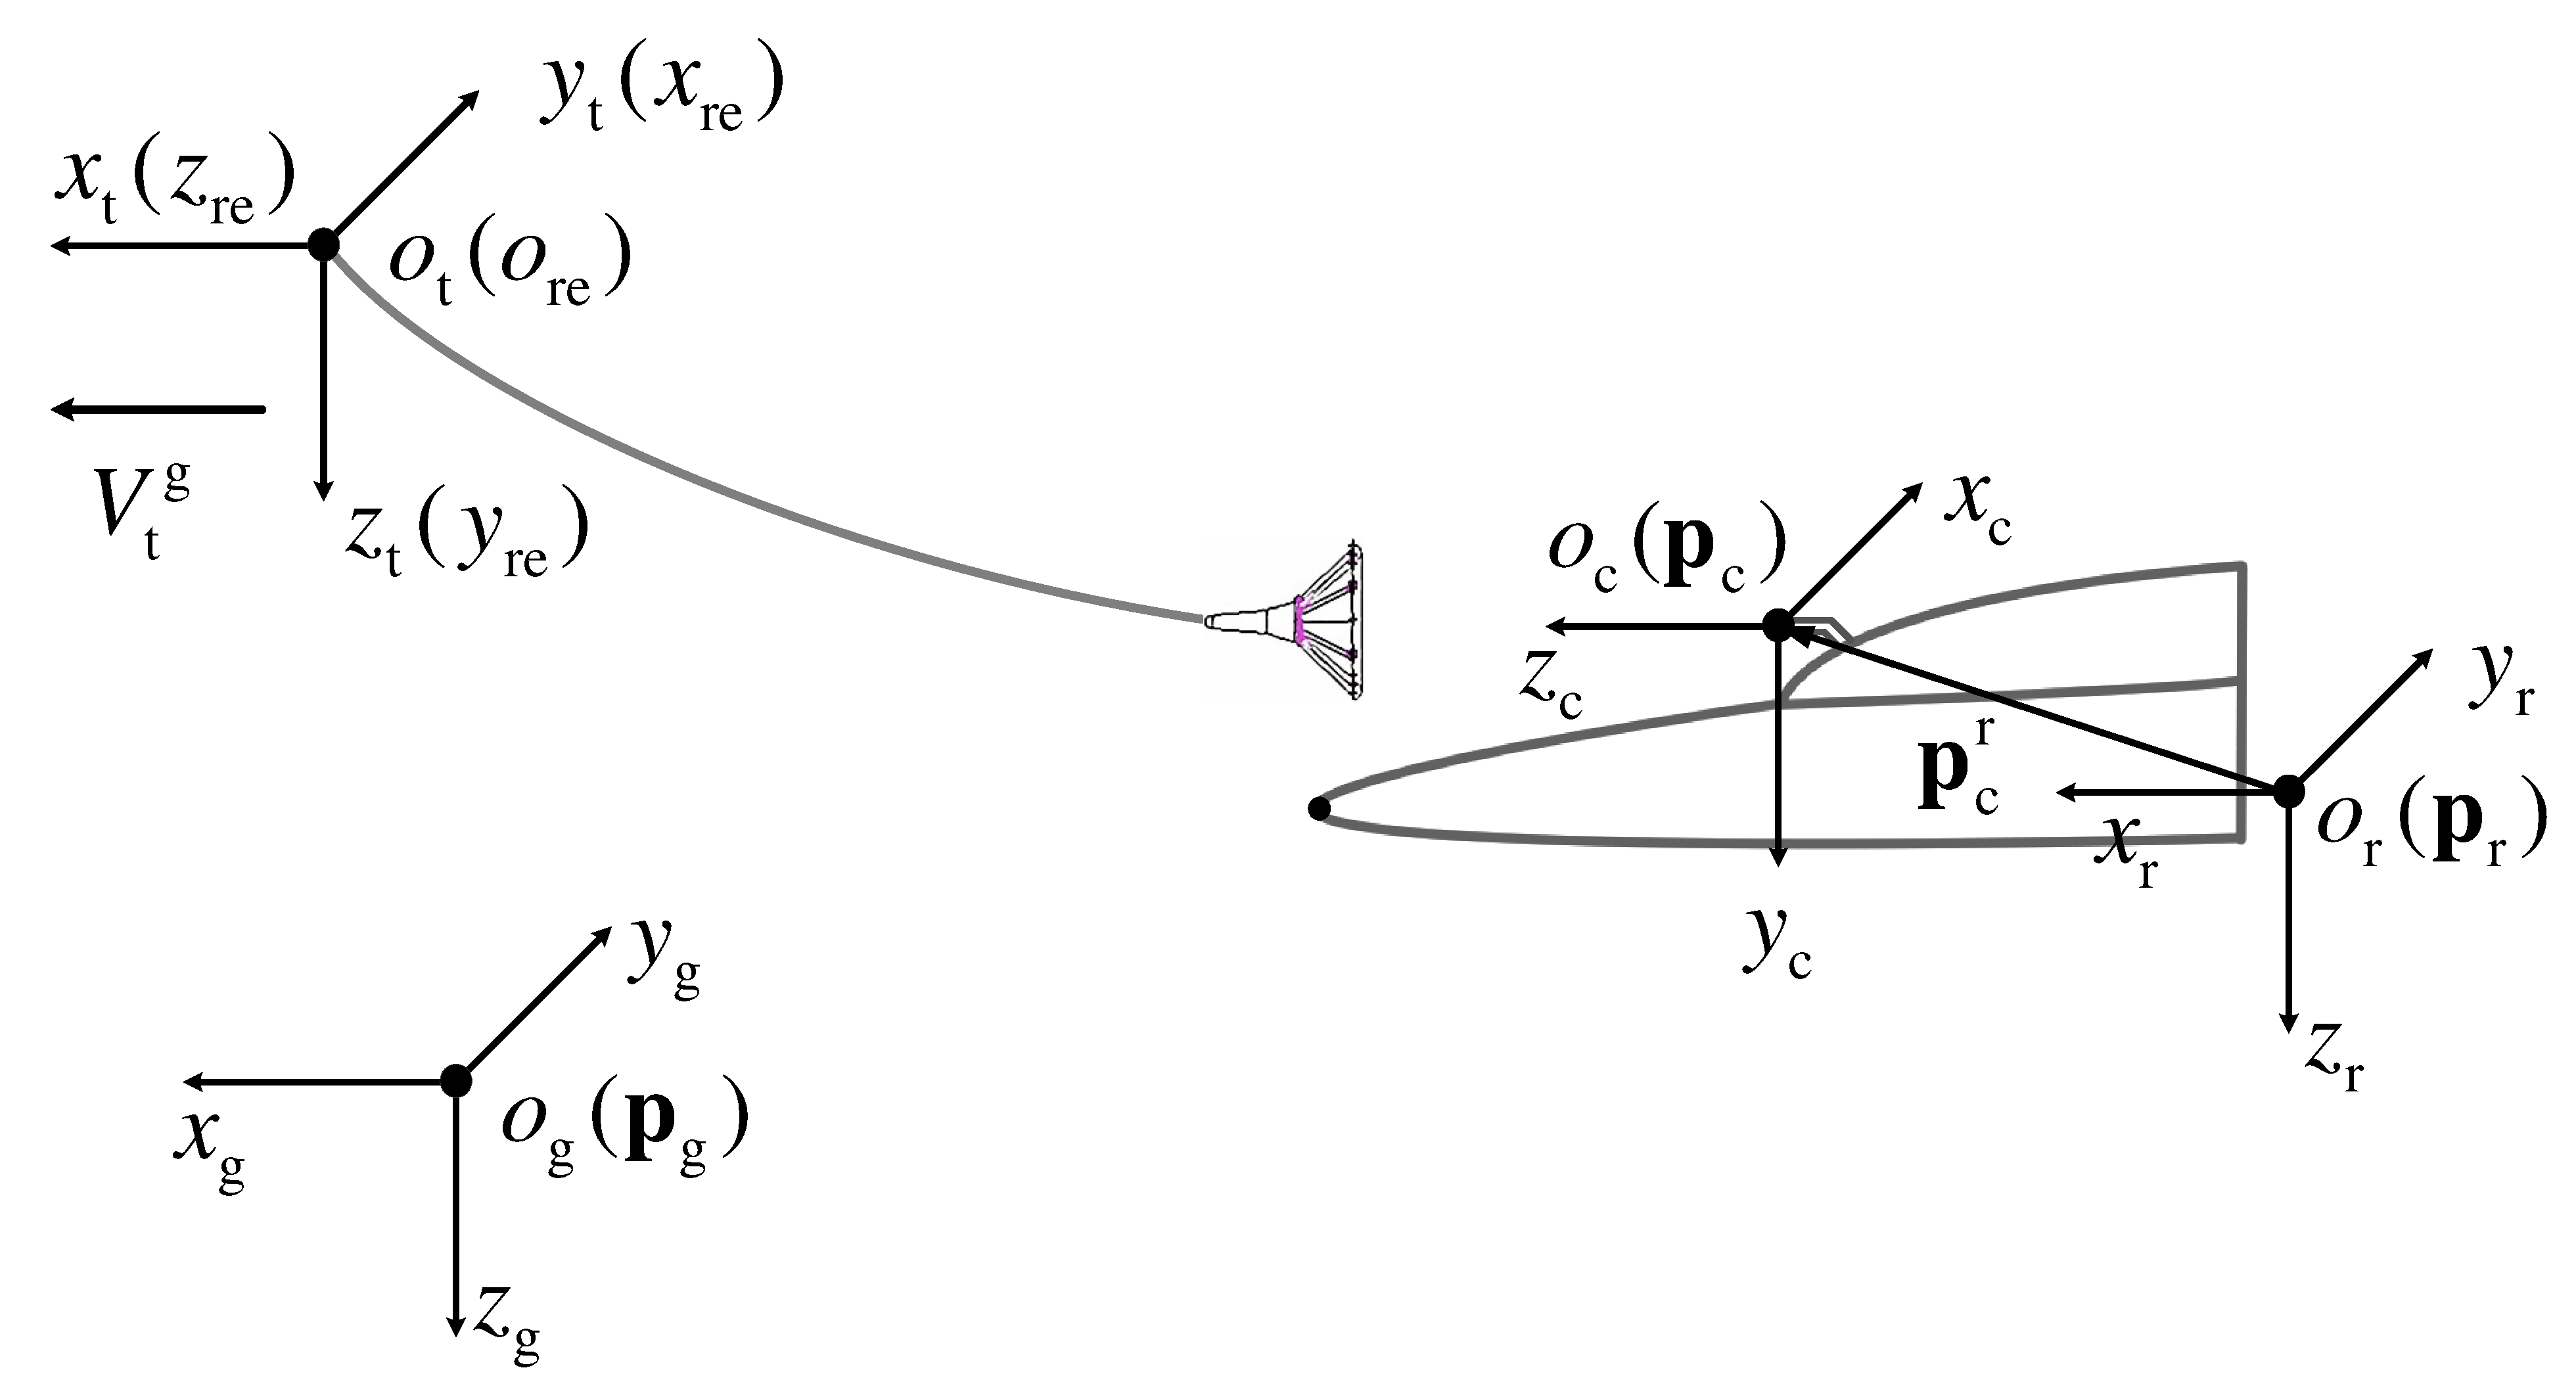
\includegraphics[width=.5\textwidth]{Figures/Figs_Ch11/fig1.pdf}
	\caption{Coordinate frames used in the PDR docking process}\label{fig1}
\end{figure}

During the docking stage, the receiver performs a level flight. Motion equations of the receiver \cite{beard2012small} under the tanker coordinate frame are decoupled into a longitudinal motion that does not depend on lateral states
\begin{equation}
\left\{ \begin{aligned}
{{\dot x}_{\rm{r}}} =& {V_{\rm{r}}}^{\rm{g}}\cos \left( {\theta  - \alpha } \right) \hfill \\
{{\dot h}_{\rm{r}}} =& {V_{\rm{r}}}^{\rm{g}}\sin \left( {\theta  - \alpha } \right) \hfill \\
\dot \theta  =& q \hfill \\
{{\dot V}^{\rm{g}}_{\rm{r}}} =& {{T\cos \alpha } \mathord{\left/
		{\vphantom {{{F_{\rm{T}}}\cos \alpha } m}} \right.
		\kern-\nulldelimiterspace} m} - {D \mathord{\left/
		{\vphantom {D m}} \right.
		\kern-\nulldelimiterspace} m} - g\left( {\cos \alpha \sin \theta  - \sin \alpha \cos \theta } \right) \hfill \\
\dot \alpha  = & - {{T\sin \alpha } \mathord{\left/
		{\vphantom {{m{V_{\rm{r}}^{\rm{g}}}}}} \right.
		\kern-\nulldelimiterspace} {m{V_{\rm{r}}}}}^{\rm{g}} - {L \mathord{\left/
		{\vphantom {L {m{V_{\rm{r}}}}}} \right.
		\kern-\nulldelimiterspace} {m{V_{\rm{r}}}}}^{\rm{g}} + q \\
& + {{g\left( {\sin \alpha \sin \theta  + \cos \alpha \cos \theta } \right)} \mathord{\left/
		{\vphantom {{g\left( {\sin \alpha \sin \theta  + \cos \alpha \cos \theta } \right)} {{V^{\rm{g}}_{\rm{r}}}}}} \right.
		\kern-\nulldelimiterspace} {{V^{\rm{g}}_{\rm{r}}}}} \hfill \\
\dot q =& {c_7} \bar M \hfill \\ 
\end{aligned}  \right. \label{eq1}
\end{equation}
and the corresponding lateral motion
\begin{equation}
\left\{ \begin{aligned}
&	{{\dot y}_{\rm{r}}} = {V_{\rm{r}}}^{\rm{g}}\cos \left( {\theta  - \alpha } \right)\sin \left( {\psi  + \beta } \right) \hfill \\
&\dot \psi  = {{\left( {q\sin \phi  + r\cos \phi } \right)} \mathord{\left/
		{\vphantom {{\left( {q\sin \phi  + r\cos \phi } \right)} {\cos \theta }}} \right.
		\kern-\nulldelimiterspace} {\cos \theta }} \hfill \\
&	\dot \phi  = p + \tan \theta \left( {q\sin \phi  + r\cos \phi } \right) \hfill \\
&\dot \beta  = {{\bar Y} \mathord{\left/
		{\vphantom {{\bar Y} {m{V_{\rm{r}}^{\rm{g}}}}}} \right.
		\kern-\nulldelimiterspace} {m{V_{\rm{r}}}^{\rm{g}}}} + p\sin \alpha  - r\cos \alpha  \hfill \\
&	\dot p = \left( {{c_1}r + {c_2}p} \right)q + {c_3}\bar L + {c_4} { N }  \hfill \\
&\dot r = \left( {{c_8}p - {c_2}r} \right)q + {c_4}\bar L + {c_9} { N  } \hfill \\ 
\end{aligned}  \right. \label{eq2}
\end{equation}
where the lift, drag, and thrust forces, the roll, pitch, and yaw moments, and the aerodynamic side force
are denoted by $ L $, $ D $, $ T $, $ \bar L $,  $ \bar M $, $ N $, and $ \bar Y $, respectively. Besides, $ c_{1} $ - $ c_{9} $ denote the inertia moment and inertia product components. Eqs. (\ref{eq1}) and (\ref{eq2}) can be simply represented as
\begin{equation}
\dot{\mathbf{x} }  _{\rm{r}} =\mathbf{f} \left ( \mathbf{x} _{\rm{r}} ,  \mathbf{u} _{\rm{r}}  \right ) \label{eq3}
\end{equation}
where ${\mathbf{x} }  _{\rm{r}} =$ [ $ {{x_{\rm{r}}}} $  $ {{y_{\rm{r}}}}  $ ${{h_{\rm{r}}}} $ $ \phi $ $ \theta $ $ \psi $ $ {{V_{\rm{r}} ^{\rm{g}}}}$ $ \alpha $ $ \beta $ $ p $ $ q $ $ r $ 
]$ ^{\text{T}} $
denotes the receiver's state, which comprises position, Euler angles, speed, aerodynamic angles, and angular rates. The vector  $ \textbf{{u}}\rm{_{r}}= $ [
$ 	{\delta}_{\rm{t}} $   $ {\delta}_{\rm{e}} $  $ {\delta}_{\rm{a}} $  $ {\delta}_{\rm{r}}  $
] $ ^{\text{T}} $
denotes the control input, which comprises the throttle, elevator, aileron, and rudder inputs. 


It is challenging to design a control law directly for the decoupled nonlinear models (\ref{eq1}) and (\ref{eq2}), so it is necessary to linearize and simplify the nonlinear models accordingly. Trimming should be considered before linearizing to obtain the equilibrium point of the nonlinear models by balancing the aerodynamic forces and moments  of the receiver in a certain state.
The process of trimming is to solve the trim states and inputs of Eq. (\ref{eq3}). In general, trim conditions can be expressed as
\begin{equation}
\dot{\mathbf{x} } ^{\ast } _{\rm{r}} =\mathbf{f} \left ( \mathbf{x}^{\ast } _{\rm{r}} ,  \mathbf{u}^{\ast } _{\rm{r}}  \right ) \label{eq4} 
\end{equation}
where $ {\textbf{x}}_{\rm{r}}^ * $ denotes the trim state and $ {\textbf{u}}_{\rm{r}}^ * $ denotes the trim input.  Here, the trim conditions are selected with respect to the state of the tanker $ \textbf{v}_{\rm{t}}^{\rm{\ast}}= $ [ $ {V}^{\rm{g}}_{\rm{t}} $ $ 0 $ $ 0 $]$ ^{\rm{T}} $, and the results can be calculated by the numerical method \cite{stevens2015aircraft}. 

As for the nonlinear model $ \dot{\mathbf{x} }  _{\rm{r}} =\mathbf{f} \left ( \mathbf{x} _{\rm{r}} ,  \mathbf{u} _{\rm{r}}  \right ) $, under the equilibrium point $ \left ( \mathbf{x} _{\rm{r}}^{\ast } ,  \mathbf{u} _{\rm{r}}^{\ast }  \right ) $, define $\tilde{\mathbf{x} } _{\rm{r}}\triangleq  \mathbf{x} _{\rm{r}}-\mathbf{x} _{\rm{r}}^{*} $ and $\tilde{\mathbf{u} } _{\rm{r}}\triangleq  \mathbf{u} _{\rm{r}}-\mathbf{u} _{\rm{r}}^{*}  $. Then, by using Taylor series expansion at the equilibrium point and retaining  only the primary term, the linear model of the receiver is obtained as
\begin{equation}
\dot{\tilde{\mathbf{x } }}  _{\rm{r}}=  \mathbf{A} \tilde{\mathbf{x } }_{\rm{r}}+  \mathbf{B} \tilde{\mathbf{u } }_{\rm{r}} \label{eq5}
\end{equation}
where $ \mathbf{A} =\frac{\partial \mathbf{f\left ( \mathbf{x}_{\rm{r}} , \mathbf{u}_{\rm{r}} \right ) } }{\partial \mathbf{x}_{\rm{r}}}\mid_{ \mathbf{x}_{\rm{r}}=\mathbf{x}_{\rm{r}}^{\ast }, \mathbf{u}_{\rm{r}}=\mathbf{u}_{\rm{r}}^{\ast }} ,\mathbf{B}= \frac{\partial \mathbf{f\left ( \mathbf{x}_{\rm{r}} , \mathbf{u}_{\rm{r}} \right ) } }{\partial \mathbf{u}_{\rm{r}}}\mid_{ \mathbf{x}_{\rm{r}}=\mathbf{x}_{\rm{r}}^{\ast }, \mathbf{u}_{\rm{r}}=\mathbf{u}_{\rm{r}}^{\ast }} $. Furthermore, according to Eq. (\ref{eq5}), the decoupled models (\ref{eq1}) and (\ref{eq2}) become
\begin{equation}
\left\{ \begin{aligned}
\mathbf{\dot{\tilde{\rm{x}} }} _{\rm{rlon}} &=\rm{\mathbf{A} }_{rlon} \tilde{\mathbf{\rm{x}} } _{\rm{rlon}}+\rm{\mathbf{B} }_{rlon}\tilde{\mathbf{\rm{u}} } _{\rm{rlon}}  \\  
\dot{\tilde{\mathbf{\rm{x}} } } _{\rm{rlat}} &=\rm{\mathbf{A} }_{rlat} \tilde{\mathbf{\rm{x}} } _{\rm{rlat}}+\rm{\mathbf{B} }_{rlat}\tilde{\mathbf{\rm{u}} } _{\rm{rlat}} 
\end{aligned}\right.  \label{eq6}
\end{equation}
where $ \tilde{\mathbf{u}}\rm{_{rlon}}=$ [ $  \tilde{\delta}_{\rm{a}} $   $  \tilde{\delta}_{\rm{r}}  $ ]
$ ^{\text{T}} $
, $ \tilde{\mathbf{u}}\rm{_{rlat}}=$[ $ \tilde{\delta}_{\rm{e}} $   $ \tilde{\delta}_{\rm{t}}  $ ]
$ ^{\text{T}} $, $ \tilde{\mathbf{\rm{x} } } _{\rm{rlon}} =$ [ $ \tilde{x}_{\rm{r}} $  $ \tilde{h}_{\rm{r}} $   $ \tilde{\theta} $ $ \tilde{{V}}^{\rm{g}}_{\rm{r}} $ $ \tilde{\alpha} $   $  \tilde{q} $ ]$ ^{\rm{T}} $ and $ \tilde{\mathbf{\rm{x}} }_{\rm{rlat}}=$ [ $ \tilde{y}_{\rm{r}} $ $ \tilde{\psi} $  $ \tilde{\phi} $   $ \tilde{\beta} $  $ \tilde{p} $ $ \tilde{r} $ ] $ ^{\rm{T}} $. Here, the subscripts ``rlon'' and ``rlat'' refer to the longitudinal and lateral channels of the receiver, respectively. Besides, $ \textbf{A}\rm{_{rlon}} $, $\textbf{A}\rm{_{rlat}} $, $ \textbf{B}\rm{_{rlon}} $, $ \textbf{B}\rm{_{rlat}} $ are known time-invariant matrices with appropriate dimensions.


\subsection{Camera Pinhole Model}
\begin{figure}[hbt!]
	\centering
	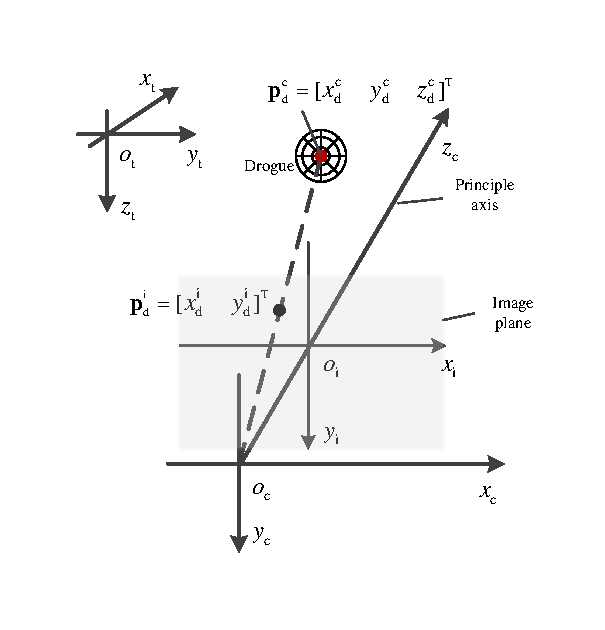
\includegraphics[width=.4\textwidth]{Figures/Figs_Ch11/fig2.pdf}
	\caption{Camera pinhole model. $ o_{\rm{t}}x_{\rm{t}}y_{\rm{t}}z_{\rm{t}}$ is the tanker coordinate frame; $ o_{\rm{c}}x_{\rm{c}}y_{\rm{c}}z_{\rm{c}}$ is the camera coordinate frame; $ o_{\rm{i}}x_{\rm{i}}y_{\rm{i}}$ is the image coordinate  frame.}\label{fig2}
\end{figure}
Assume that a vector $ \mathbf{p}^{\rm{i}}_{\rm{d}} =$ [ $ x^{\rm{i}}_{\rm{d}} $ $ y^{\rm{i}}_{\rm{d}} $ ] $ ^{\rm{T}}$ is in the image coordinate system $o_{\mathrm{i}}-x_{\mathrm{i}}y_{\mathrm{i}}$. $\mathbf{p}^{\mathrm{c}}_{\mathrm{d}}$ and $\mathbf{p}^{\mathrm{t}}_{\mathrm{d}}$ can be transformed to $\mathbf{p}^{\rm{i}}_{\rm{d}}$ by using the camera pinhole model \cite{sun2019bionic,yan2018vision} (see Fig.~\ref{fig2})  as follows 
\begin{equation}
s\!\begin{bmatrix}\!  x^{\rm{i}}_{\rm{d}}  \\  y^{\rm{i}}_{\rm{d}}  \\ 1\!\end{bmatrix}\!\!= \!\!\begin{bmatrix}\!
\alpha _{\mathrm{x}} & 0 & u_{\mathrm{0}} & 0 \\ 0 & \alpha _{\mathrm{y}} & v_{\mathrm{0}} & 0 \\ 0 & 0 & 1 &
0\!\end{bmatrix}\!\!\begin{bmatrix}\! x^{\rm{c}}_{\mathrm{d}} \\ y^{\rm{c}}_{\mathrm{d}} \\ z^{\rm{c}}_{\mathrm{d}} \\ 1\!\end{bmatrix}\!\\
\!=\!\mathbf{M}\!\begin{bmatrix}\! \mathbf{R}_{\rm{t}}^{\rm{c}} &
\mathbf{t}_{\rm{t}}^{\rm{c}} \\ 0 & 1\!\end{bmatrix}\!\!\begin{bmatrix}\! x^{\rm{t}}_{\mathrm{d}} \\
y^{\rm{t}}_{\mathrm{d}} \\ z^{\rm{t}}_{\mathrm{d}} \\ 1\!\end{bmatrix}\!   \label{eqCam}
\end{equation}%
and
\begin{equation}
\mathbf{M}=
\begin{bmatrix}
\alpha _{\mathrm{x}} & 0 & u_{\mathrm{0}} \\ 
0 & \alpha _{\mathrm{y}} & v_{\mathrm{0}} \\ 
0 & 0 & 1
\end{bmatrix}
\label{eqCam2}
\end{equation}
where $s$ in~(\ref{eqCam}) is the scaling factor.  $\mathbf{R}_{\mathrm{t}}^{\mathrm{c}}\in \mathbf{R}^{3\times 3}$ is the rotation matrix from the tanker frame to the camera frame, and $\mathbf{t}_{\mathrm{t}}^{\mathrm{c}}\in \mathbf{R}^{3}$ is the translation vector from the tanker frame to the camera frame. $\mathbf{M}$ is the camera intrinsic
matrix, and its elements $\alpha _{\mathrm{x}}$, $\alpha _{\mathrm{y}}$, $u_{\mathrm{0}}$ and $v_{\mathrm{0}}$ are
determined by camera calibration \cite{7738351}.

In the PBVS control, the position information of the drogue $\mathbf{p}^{\rm{t}}_{\rm{d}}=\!\begin{bmatrix}\! x^{\rm{t}}_{\mathrm{d}} &
y^{\rm{t}}_{\mathrm{d}} & z^{\rm{t}}_{\mathrm{d}} \end{bmatrix}\!^{\text{T}} $  needs be obtained based on the relationship decribed in Eq.~(\ref{eqCam}), and the detailed calculation procedure can be found in \cite{yan2018vision}.
If there exist pointing errors of the camera, $\mathbf{R}_{\mathrm{t}}^{\mathrm{c}}\in \mathbf{R}^{3\times 3}$ will be incorrect. If there exist installation position errors of the camera, $\mathbf{t}_{\mathrm{t}}^{\mathrm{c}}\in \mathbf{R}^{3}$ will be incorrect. As a result, the obtained position information of the drogue will be incorrect, which will affect the control performance of the PBVS control. On the contrary, the IBVS control adopts image information $ \mathbf{p}^{\rm{i}}_{\rm{d}} =$ [ $ x^{\rm{i}}_{\rm{d}} $ $ y^{\rm{i}}_{\rm{d}} $ ] $ ^{\rm{T}}$ rather than position information to design a docking controller, which is more robust against the pose estimation error.


\subsection{Problem Formulation}
In this paper, the situation is considered that a forward-looking monocular camera is mounted on the probe tip of the receiver. The drogue image is the emphasis in the visual servo control for PDR. Define the coordinate of the drogue center in the camera coordinate frame as $ \mathbf{p}^{\rm{c}}_{\rm{d}}= $ [ $ x^{\rm{c}}_{\rm{d}} $  $ y^{\rm{c}}_{\rm{d}} $ $ z^{\rm{c}}_{\rm{d}} $ ]$ ^{\rm{T}} $, which is projected in the image as a 2D point with coordinates $ \mathbf{p}^{\rm{i}}_{\rm{d}} =$ [ $ x^{\rm{i}}_{\rm{d}} $ $ y^{\rm{i}}_{\rm{d}} $ ] $ ^{\rm{T}}$ as shown in Fig. \ref{fig2}. 
The image tracking error is defined as 
\begin{equation}
\mathbf{e}=\begin{bmatrix}
e_{x} \\
e_{y} 
\end{bmatrix}=\begin{bmatrix}
x^{\rm{i}}_{\rm{d}}-x_{\rm{o}}^{\rm{i}} \\
y^{\rm{i}}_{\rm{d}}-y_{\rm{o}}^{\rm{i}}
\end{bmatrix} \label{eq7}
\end{equation}
where $ \left (x_{\rm{o}}^{\rm{i}}, y_{\rm{o}}^{\rm{i}}\right )$ is the convergence point of the drogue image, which is the origin of the image frame here. 

Besides, the docking depth $  z^{\rm{c}}_{\rm{d}}$, as shown in Fig. \ref{fig3}, is the position difference between the camera and the plane of the drogue center (where LEDs are installed) along the $ z_{\rm{c}} $ axis. After the image tracking error converges to zero, in order to achieve a successful docking, the docking depth $  z^{\rm{c}}_{\rm{d}}$ also needs to be controlled to zero, meanwhile ensuring the docking velocity within the required range 1-1.5m/s \cite{NATO-2004-3} at the docking moment. 

\begin{figure}[hbt!]
	\centering
	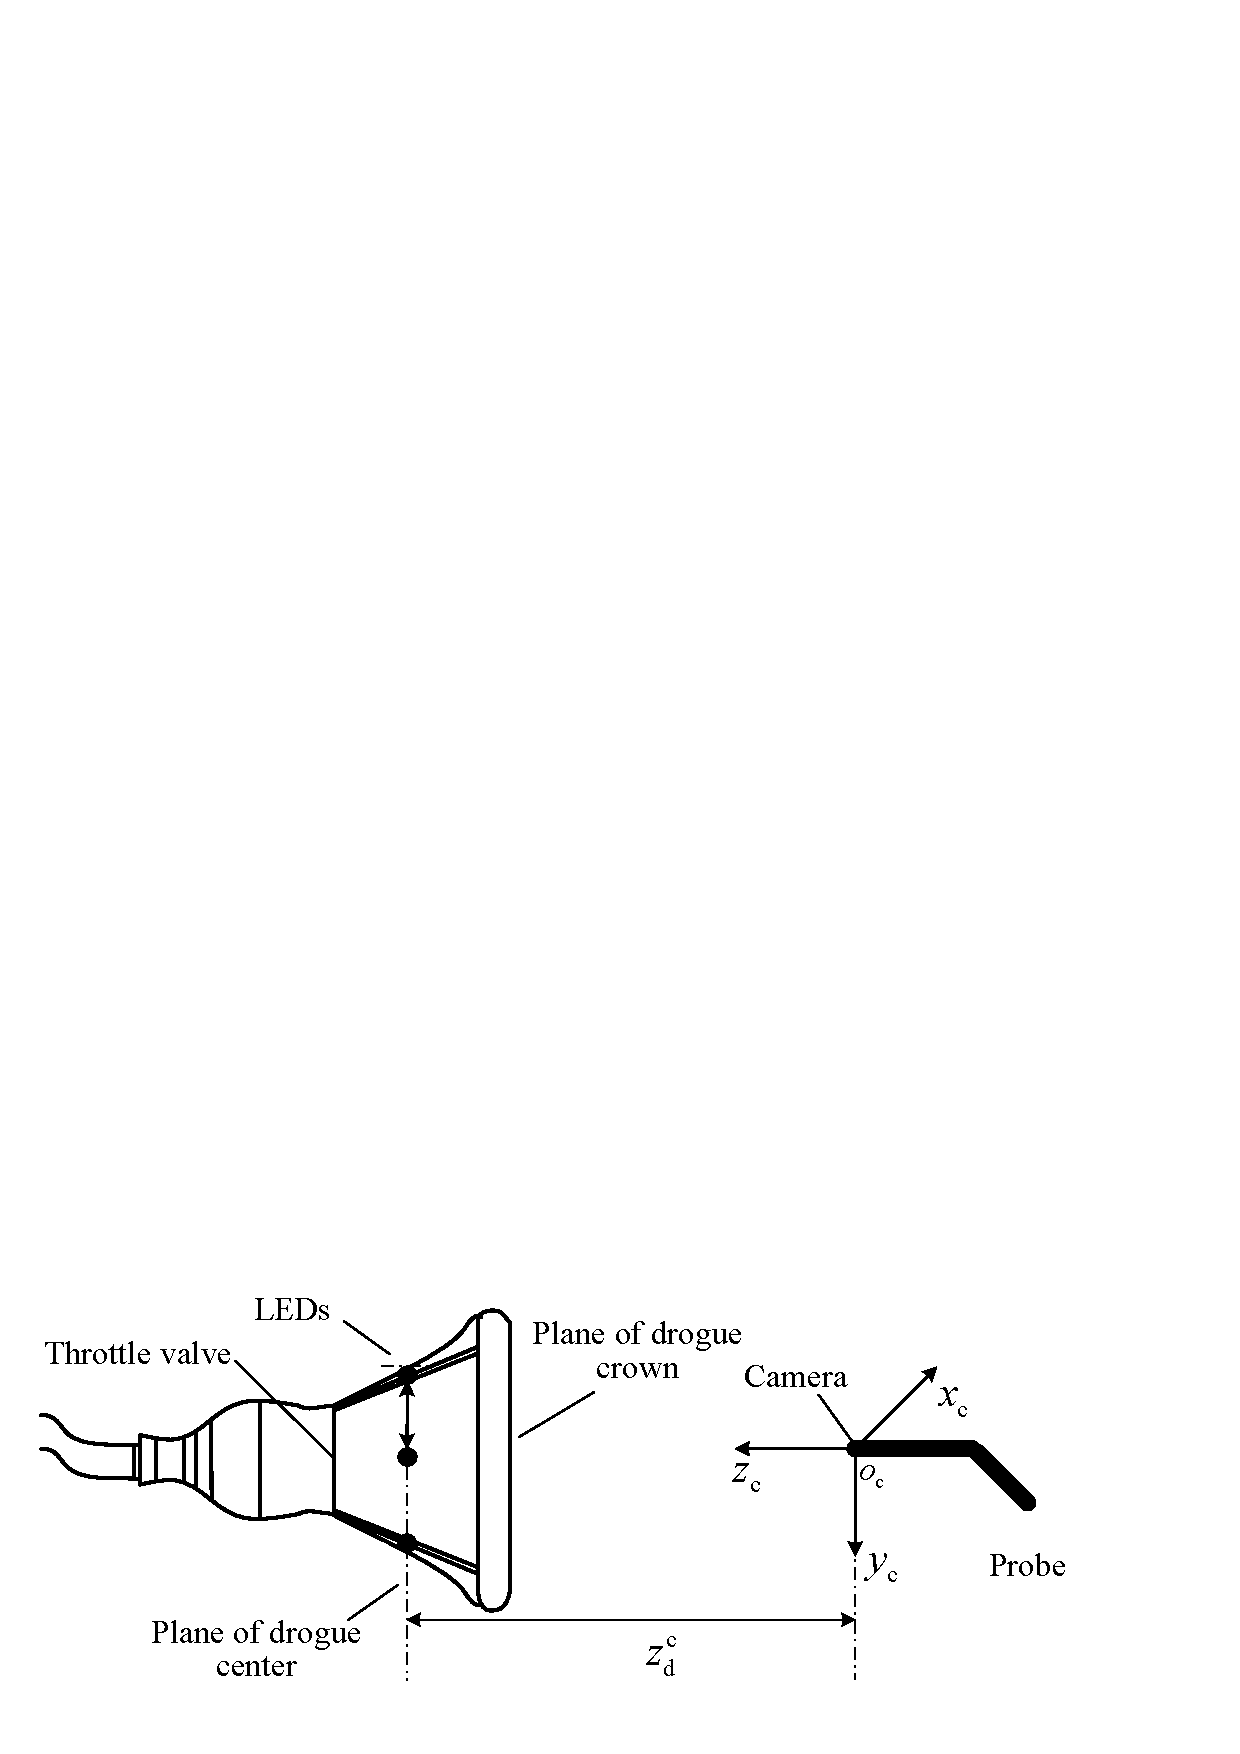
\includegraphics[width=.5\textwidth]{Figures/Figs_Ch11/fig3.pdf}
	\caption{Schematic diagram of docking depth.} \label{fig3}
\end{figure} 

In image-based visual servo, except for the image tracking error, the docking depth must be obtained. Laser distance measuring technology is commonly adopted \cite{xie2008switching}. In this study, the docking depth is acquired using the pinhole imaging principle \cite{yan2018vision}. According to the pinhole imaging principle, one has
\begin{equation}
\frac{R_{{\rm{dr}}}}{{z^{\rm{c}}_{\rm{d}} }} = \frac{r}{f} \label{eq8}
\end{equation}
where $R_{{\rm{dr}}}$ is the actual drogue radius, $r$ is the drogue radius in the image, $f$ is the focal length of the adopted monocular camera. Thus, the docking depth is determined as
\begin{equation}
z^{\rm{c}}_{\rm{d}} = \frac{{{R_{{\rm{dr}}}}f}}{r}  \label{eq9}
\end{equation}
On the whole, after the camera data processing, one can obtain the spatial errors $e_x$, $e_y$ and the docking depth $z^{\rm{c}}_{\rm{d}}$, which will be used in the feedback controller design later.


Before proceeding further, four assumptions are made in the following.

\textbf{Assumption 1.}
The visual tracking module of the receiver can accurately capture the drogue's central coordinate $  \textbf{p}^{\rm{i}}_{\rm{d}} $ from images in real time.


\textbf{Assumption 2.}
The tanker is in a steady flight during the entire docking process, while the receiver keeps a certain distance relative to the tanker with the trim state $ \textbf{v}_{\rm{r}}^{\rm{\ast}}= \textbf{v}_{\rm{t}}^{\rm{\ast}}$.


\textbf{Assumption 3.}    
During the docking process, the pitch, roll, and yaw angles of the receiver are small.

\textbf{Assumption 4.}   
The camera installation position coincides with the probe tip, as shown in Fig. \ref{fig1}. The transformation matrix from the tanker coordinate frame to the camera coordinate frame is 
\begin{equation}
\mathbf{R} \rm{_{c/t}}=\begin{bmatrix}
0 &1  &0 \\
0&0 & 1\\
1 & 0 &0
\end{bmatrix}. \label{eq10}
\end{equation}


Based on \textit{Assumptions 1-4}, the \textit{Visual Servo Control Problem} for the PDR docking is to design a proper control input $ \tilde{\mathbf{u}}\rm{_{r}}=$ [ $  \tilde{\delta}_{\rm{a}} $   $  \tilde{\delta}_{\rm{r}}  $ $ \tilde{\delta}_{\rm{e}} $  $ \tilde{\delta}_{\rm{t}}$ ]
$ ^{\text{T}} $
for system (\ref{eq6}) to make the image tracking error converge to zero $ \left ( \mathbf{e}(t) \to 0 \right )  $  as $ t\to\infty  $ and the depth error converge to zero $ \left ( z^{\rm{c}}_{\rm{d}}(t) \to 0 \right )$ slower than $ \left ( \mathbf{e}(t) \to 0 \right )  $.
\section{IBVS controller design}
In this section, an IBVS model with a forward-looking monocular camera mounted on the receiver is established, which describes the relationship between image errors and the camera's linear and angular velocities, and the relationship between the camera's motion and the receiver's motion. Besides, based on the obtained model, an IBVS controller is designed.

\subsection{Outer-loop visual servo model based on the Jacobian matrix}


By applying the basic equation of IBVS \cite{chaumette2006visual} in the PDR system, the relationship between $ \mathbf{e}  $ and $ \textbf{v}^{\rm{c}}_{\rm{d}} $, $ \mathbf{\omega}^{\rm{c}}_{\rm{d}} $ is
\begin{equation}
\begin{split}
&\dot{\mathbf{e}}=\\
&\underbrace{\begin{bmatrix}
	-\frac{1}{z_{\rm{d}}^{\rm{c}} } & 0 &\frac{x_{\rm{d}}^{\rm{i}} }{z_{\rm{d}}^{\rm{c}} }   & x_{\rm{d}}^{\rm{i}}y_{\rm{d}}^{\rm{i}}   & -(1+{x_{\rm{d}}^{\rm{i}}}^{2} ) & y_{\rm{d}}^{\rm{i}} \\
	0& -\frac{1}{z_{\rm{d}}^{\rm{c}}}  & \frac{y_{\rm{d}}^{\rm{i}} }{z_{\rm{d}}^{\rm{c}}}  &1+{y_{\rm{d}}^{\rm{i}}}^{2}   &-x_{\rm{d}}^{\rm{i}}y_{\rm{d}}^{\rm{i}}    &-x_{\rm{d}}^{\rm{i}}
	\end{bmatrix}}_{\mathbf{L}} \underbrace{\left [\begin{matrix} v^{\rm{c}}_{\rm{d},x} \\  v^{\rm{c}}_{\rm{d},y} \\ v^{\rm{c}}_{\rm{d},z} \\ \omega^{\rm{c}}_{\rm{d},x} \\ \omega^{\rm{c}}_{\rm{d},y} \\ \omega^{\rm{c}}_{\rm{d},z}\end{matrix}\right ] }_{\mathbf{u}^{\rm{c}}_{\rm{d}}} 
\end{split} \label{eq11}
\end{equation}
where  $\textbf{L} \in {\mathbb{R}^{2 \times 6}}$ is the Jacobian matrix, ${\mathbf{{u}}^{\rm{c}}_{\rm{d}}}= $ [ $ (\mathbf{v}_{\rm{d}}^{\rm{c}})^{\rm{T}} $ $(\mathbf{\omega}_{\rm{d}}^{\rm{c}})^{\rm{T}}  $ ]$ ^{\rm{T}} $ with 
$ \mathbf{v}_{\rm{d}}^{\rm{c}}=$ [ $ v^{\rm{c}}_{{\rm{d}},x} $ $ v^{\rm{c}}_{{\rm{d}},y} $ $ v^{\rm{c}}_{{\rm{d}},z} $ ]$ ^{\rm{T}} $ $=\textbf{v}_{\rm{d}}^{\rm{t}}-\textbf{v}_{\rm{c}}^{\rm{t}}=\textbf{v}_{\rm{d}}^{\rm{re}}-\textbf{v}_{\rm{c}}^{\rm{re}}$ and $ \mathbf{\omega}_{\rm{d}}^{\rm{c}}=$ [ $ \omega^{\rm{c}}_{{\rm{d}},x} $ $ \omega^{\rm{c}}_{{\rm{d}},y} $ $ \omega^{\rm{c}}_{{\rm{d}},z} $]$ ^{\rm{T}} $ are the drogue velocity and angular velocity in the camera coordinate frame. Specially, $ \textbf{v}_{\rm{c}}^{\rm{re}} =$ [ $ v^{\rm{re}}_{{\rm{c}},x} $ $ v^{\rm{re}}_{{\rm{c}},y} $ $ v^{\rm{re}}_{{\rm{c}},z} $ ]$ ^{\rm{T}} $  and $ \textbf{v}_{\rm{d}}^{\rm{re}} $ are the velocity of the camera and the drogue under the reference coordinate frame.
In order to simplify the later controller design, Eq. (\ref{eq11}) is further decomposed into a longitudinal channel and a lateral channel.
\begin{itemize}
	\item Longitudinal channel:
	In the $ x_{\rm{c}}-z_{\rm{c}} $ plane, state variables are $ {v}_{{\rm{d}},x}^{\rm{c}} $, $ {v}_{{\rm{d}},z}^{\rm{c}} $, $ {\omega}_{{\rm{d}},y}^{\rm{c}} $ with $ {v}_{{\rm{d}},y}^{\rm{c}}=0 $, $ {\omega}_{{\rm{d}},x}^{\rm{c}}=0 $, $ {\omega}_{{\rm{d}},z}^{\rm{c}}=0 $. One can obtain 
	\begin{equation}
	\dot{e}_{x}=-\frac{{v}_{{\rm{d}},x}^{\rm{c}} }{{z}_{\rm{d}}^{\rm{c}} } +\frac{e_{x}{v}^{\rm{c}}_{{\rm{d}},z} }{{z}_{\rm{d}}^{\rm{c}} } -(1+e_{x}^{2} ){\omega}_{{\rm{d}},y}^{\rm{c}}. \label{eq12}
	\end{equation}
	\item Lateral channel:
	In the $ y_{\rm{c}}-z_{\rm{c}} $ plane, state variables are $ {v}_{{\rm{d}},y}^{\rm{c}} $, $ {v}_{{\rm{d}},z}^{\rm{c}} $, $ {\omega}_{{\rm{d}},x}^{\rm{c}} $ with $ {v}_{{\rm{d}},x}^{\rm{c}}=0 $, $ {\omega}_{{\rm{d}},y}^{\rm{c}}=0 $, $ {\omega}_{{\rm{d}},z}^{\rm{c}}=0 $. One can obtain 
	\begin{equation}
	\dot{e}_{y}=-\frac{{v}_{{\rm{d}},y}^{\rm{c}} }{{z}_{\rm{d}}^{\rm{c}} } +\frac{e_{y}{v}_{{\rm{d}},z}^{\rm{c}} }{ {z}_{\rm{d}}^{\rm{c}} } -(1+e_{y}^{2} ){\omega}_{{\rm{d}},x} ^{\rm{c}}. \label{eq13}
	\end{equation}
\end{itemize}


\subsection{Inner-loop dynamic model}

For the Jacobian matrix based visual servo model (\ref{eq11}), the input variable is $ \mathbf{v}_{\rm{d}}^{\rm{c}}=$ [ $ v^{\rm{c}}_{{\rm{d}},x} $ $ v^{\rm{c}}_{{\rm{d}},y} $ $ v^{\rm{c}}_{{\rm{d}},z} $ ]$ ^{\rm{T}} $ based on that the change of $ \mathbf{\omega}_{\rm{d}}^{\rm{c}}=$ [ $ \omega^{\rm{c}}_{{\rm{d}},x} $ $ \omega^{\rm{c}}_{{\rm{d}},y} $ $ \omega^{\rm{c}}_{{\rm{d}},z} $]$ ^{\rm{T}} $ is small in the docking process which can be ignored. In practice, since $ \textbf{v}_{\rm{d}}^{\rm{c}}=\textbf{v}_{\rm{d}}^{\rm{re}}-\textbf{v}_{\rm{c}}^{\rm{re}} $, one can only control $ \textbf{v}_{\rm{c}}^{\rm{re}} $ rather than $ \textbf{v}_{\rm{d}}^{\rm{re}} $, because $ \textbf{v}_{\rm{d}}^{\rm{re}} $ is the dynamics of the drogue, which is passive. Thus, the camera motion needs to be controlled, which is indirectly controlled by the receiver. Roughly,  $ \textbf{v}_{\rm{c},des}^{\rm{re}}=-\textbf{v}_{{\rm{d}},\rm{des}}^{\rm{c}}  $ will be used by  taking $ \textbf{v}_{\rm{d}}^{\rm{re}} $ as a disturbance, which is expressed in a decoupled form as
\begin{equation}
{\textbf{v}}^{\rm{re}}_{\rm{c,des}}=\begin{bmatrix}
{\textbf{v}}_{\rm{rlon},des}^{\rm{re}}  \\
{{v}}_{\rm{rlat},des}^{\rm{re}}
\end{bmatrix} \label{eq31}
\end{equation}
where ${\textbf{v}}^{\rm{re}}_{\rm{rlon},des}=$ [${v}^{\rm{c}}_{{\rm{d}},y\rm{des}}$ 
$ {v}^{\rm{c}}_{{\rm{d}},z\rm{des}} $ ]$ ^{\rm{T}} $,  $ {v}^{\rm{re}}_{\rm{rlat},des}={v}^{\rm{c}}_{{\rm{d}},x\rm{des}} $. The task of the inner-loop controller is to make $ {\textbf{v}}_{\rm{c}}^{\rm{re}} $ track $ {\textbf{v}}_{\rm{c,des}}^{\rm{re}} $ and reject disturbances. In this part, the inner-loop dynamic model from the receiver inputs  $\tilde{\mathbf{\rm{u}} } _{\rm{rlon}} $ and  $\tilde{\mathbf{\rm{u}} } _{\rm{rlat}} $ to $\mathbf{ v}_{{\text{rlon}}}^{{\text{re}}} $ and $\mathbf{ v}_{{\text{rlat}}}^{{\text{re}}} $ will be derived. Based on the inner-loop dynamic model, the inner-loop visual servo control can then be designed. 



The receiver can be taken as a rigid body, and the camera's linear velocity is equal to the vector sum of the velocity of the receiver's center of mass and the velocity of the camera rotating around the receiver's center of mass under the tanker coordinate frame, i.e.,
\begin{equation}
\begin{split}
\mathbf{v}_{\rm{c}}^{\rm{t}}
&=\mathbf{{\omega}}_{\rm{r}}^{\rm{t}}\times \mathbf{p}_{\rm{c}}^{\rm{r}}+\mathbf{{v}}_{\rm{r}}^{\rm{t}}
\end{split} \label{eq14}
\end{equation}
where $ \mathbf{{v}}_{\rm{c}}^{\rm{t}}=[{v}^{\rm{t}}_{{\rm{c}},x} {v}^{\rm{t}}_{{\rm{c}},y} {v}^{\rm{t}}_{{\rm{c}},z}]^{\rm{T}} $ and $ \mathbf{{v}}_{\rm{r}}^{\rm{t}}=[{v}^{\rm{t}}_{{\rm{r}},x} {v}^{\rm{t}}_{{\rm{r}},y} {v}^{\rm{t}}_{{\rm{r}},z}]^{\rm{T}} $ donote the linear velocity of the camera and the receiver, $ \mathbf{{\omega}}_{\rm{r}}^{\rm{t}}=[{\omega}^{\rm{t}}_{{\rm{r}},x} {\omega}^{\rm{t}}_{{\rm{r}},y} {\omega}^{\rm{t}}_{{\rm{r}},z}]^{\rm{T}} $ denotes the angular velocity of the receiver and $ \mathbf{p}_{\rm{c}}^{\rm{r}}=$ [ $ x_{\rm{c}}^{\rm{r}} $ $ y_{\rm{c}}^{\rm{r}} $ $ z_{\rm{c}}^{\rm{r}} $ ] $^{\rm{T}} $ is the camera's coordinate under the receiver coordinate frame as shown in Fig. \ref{fig1}.

In the PDR docking, the rotation between the receiver and the tanker is kept small for safety considerations. Thus, 
the transformation matrix from the receiver coordinate frame to the tanker coordinate frame is approximated as 
\begin{equation}
\mathbf{R} \rm{_{t/r}}=\textbf{I}_{3}. \label{eq15}
\end{equation}
With Eq. (\ref{eq15}), Eq. (\ref{eq14}) becomes
\begin{equation}
\begin{split}
\mathbf{{v}}_{\rm{c}}^{\rm{t}}
&=\mathbf{{\omega}}_{\rm{r}}^{\rm{t}}\times \mathbf{p}_{\rm{c}}^{\rm{r}}+\mathbf{{v}}_{\rm{r}}^{\rm{t}}\\
&=\mathbf{R} \rm{_{t/r}}\mathbf{{\omega}}_{\rm{r}}^{\rm{r}}\times \mathbf{p}_{\rm{c}}^{\rm{r}}+\mathbf{R} \rm{_{t/r}}\mathbf{{v}}_{\rm{r}}^{\rm{r}}\\
&=\mathbf{{\omega}}_{\rm{r}}^{\rm{r}}\times \mathbf{p}_{\rm{c}}^{\rm{r}}+\mathbf{{v}}_{\rm{r}}^{\rm{r}}
\end{split} \label{eq16}
\end{equation}
where $ \mathbf{{\omega}}_{\rm{r}}^{\rm{r}}= $ [ $ \tilde{p} $ $ \tilde{q} $ $ \tilde{r} $ ] $ ^{\rm{T}} $  and $ \mathbf{{v}}_{\rm{r}}^{\rm{r}} $ = [ $ \tilde{u} $ $ \tilde{v} $ $ \tilde{w} $ ] $ ^{\rm{T}} $ . 
Based on Eq. (\ref{eq16}), the camera's linear velocity $ \textbf{v}_{\rm{c}}^{\rm{re}} $ can be expressed as
\begin{equation}
\begin{split}
\mathbf{{v}}_{\rm{c}}^{\rm{re}}
&=\mathbf{R}_{\rm{re/t}}\mathbf{{v}}_{\rm{c}}^{\rm{t}} \\
&=\mathbf{R} \rm{_{re/t}}(\mathbf{{\omega}}_{\rm{r}}^{\rm{r}}\times \mathbf{p}_{\rm{c}}^{\rm{r}}+\mathbf{{v}}_{\rm{r}}^{\rm{r}}).
\end{split}  \label{eq17}
\end{equation}
According to Ref \cite{beard2012small},  $\mathbf{{v}}_{\rm{r}}^{\rm{r}}$ can be further written as
\begin{equation}
\left\{\begin{aligned}
{\tilde{u}} &= {\tilde{V}^{\rm{g}}_{\rm{r}}}\cos \tilde{\alpha} \cos \tilde{\beta}  \\ 
{\tilde{v}} &= {\tilde{V}^{\rm{g}}_{\rm{r}}}\sin \tilde{\beta}  \\ 
{\tilde{w}} &= {\tilde{V}^{\rm{g}}_{\rm{r}}}\sin \tilde{\alpha} \cos \tilde{\beta}  \\ 
\end{aligned}\right.  \label{eq18} 
\end{equation}
Then, Eq. (\ref{eq17}) becomes 
\begin{equation}
\left\{ \begin{aligned}
{v}_{{\rm{c}},x}^{\rm{re}} &={\tilde{V}^{\rm{g}}_{\rm{r}}}\sin \tilde{\beta}+x_{\rm{c}}^{\rm{r}}\tilde{r}-z_{\rm{c}}^{\rm{r}}\tilde{p} \hfill \\
{v}_{{\rm{c}},y}^{\rm{re}} &= {\tilde{V}^{\rm{g}}_{\rm{r}}}\sin \tilde{\alpha} \cos \tilde{\beta}+ y_{\rm{c}}^{\rm{r}}\tilde{p}-x_{\rm{c}}^{\rm{r}}\tilde{q} \hfill\\
{v}_{{\rm{c}},z}^{\rm{re}} &= {\tilde{V}^{\rm{g}}_{\rm{r}}}\cos \tilde{\alpha} \cos \tilde{\beta}+ z_{\rm{c}}^{\rm{r}}\tilde{q}- y_{\rm{c}}^{\rm{r}}\tilde{r} .\hfill 
\end{aligned}  \right. \label{eq19}
\end{equation}
Based on the decoupling conditions  $\tilde{p} = \tilde{r} = 0 $, $\tilde{\beta}  = 0$ and omitting the higher-order items, Eq. (\ref{eq19}) becomes
\begin{equation}
\left\{ \begin{aligned}
v_{{\rm{c}},x}^{\text{re}} &=  x_{\rm{c}}^{\rm{r}}\tilde r - z_{\rm{c}}^{\rm{r}}\tilde p \\
v_{{\rm{c}},y}^{\text{re}} &=  - x_{\rm{c}}^{\rm{r}}\tilde q   \hfill \\
v_{{\rm{c}},z}^{\text{re}} &= {{\tilde V}_{\rm{r}}^{\rm{g}}}+z_{\rm{c}}^{\rm{r}}\tilde q.   \hfill 
\end{aligned}  \right.  \label{eq20}
\end{equation}

Combining Eq. (\ref{eq6}) and Eq. (\ref{eq20}), the longitudinal model is obtained
\begin{equation}
\left\{ \begin{aligned}
\mathbf{\dot{\tilde{\rm{x}} }} _{\rm{rlon}} &=\rm{\mathbf{A} }_{rlon} \tilde{\mathbf{\rm{x}} } _{\rm{rlon}}+\rm{\mathbf{B} }_{rlon}\tilde{\mathbf{\rm{u}} } _{\rm{rlon}}\hfill \\
\mathbf{ v}_{{\text{rlon}}}^{{\text{re}}} &=\left[ {\begin{array}{*{20}{c}}
	{ v_{{\rm{c}},y}^{\rm{re}}} \\ 
	{ v_{{\rm{c}},z}^{\rm{re}}} 
	\end{array}} \right] = \underbrace {\left[ {\begin{array}{*{20}{c}}
		0&0&0&0&0&{ - {x_{\rm{c}}^{\rm{r}}}} \\ 
		0&0&0&1&0&{{z_{\rm{c}}^{\rm{r}}}} 
		\end{array}} \right]}_{\mathbf{C}_{{\text{rlon}}}}\tilde{\mathbf{\rm{x}} } _{\rm{rlon}}
\end{aligned}  \right. \label{eq21}
\end{equation}
and the lateral model is denoted by
\begin{equation}
\left\{ \begin{aligned}
\dot{\tilde{\mathbf{\rm{x}} } } _{\rm{rlat}} &=\rm{\mathbf{A} }_{rlat} \tilde{\mathbf{\rm{x}} } _{\rm{rlat}}+\rm{\mathbf{B} }_{rlat}\tilde{\mathbf{\rm{u}} } _{\rm{rlat}}  \hfill \\
v_{{\text{rlat}}}^{{\text{re}}} &=  v_{{\rm{c}},x}^{\rm{re}} = \underbrace{\left[ {\begin{array}{*{20}{l}}
		0&0&0&0&{ -}z_{\rm{c}}^{\rm{r}}&x_{\rm{c}}^{\rm{r}}
		\end{array}} \right]}_{\textbf{C}_{{\text{rlat}}}}\tilde{\mathbf{\rm{x}} } _{\rm{rlat}}
\end{aligned}  \right. \label{eq22}
\end{equation}


\subsection{Visual servo controller design}
Based on the models (\ref{eq12}), (\ref{eq13}), (\ref{eq21}) and (\ref{eq22}), the IBVS controller design is divided into a longitudinal channel control problem and a lateral channel control problem.

\textbf{Problem 1.} (Lateral channel control). For systems  (\ref{eq13}) and (\ref{eq22}), design $ \tilde{\mathbf{\rm{u}} } _{\rm{rlat}} $, such that the lateral image tracking error converges to zero, i.e.,  $ e_{x}(t)\to 0  $ as $ t\to\infty  $.


\textbf{Problem 2.} (Longitudinal channel control). For systems (\ref{eq12}) and (\ref{eq21}), design $ \tilde{\mathbf{\rm{u}} } _{\rm{rlon}} $, such that the longitudinal image tracking error converges to zero and the probe docks with the drogue, i.e., $ e_{y}(t)\to 0  $  as $ t\to\infty  $, $ z_{\rm{d}}^{\rm{c}}(t)\to 0 $ slower than $ \left ( \mathbf{e}(t) \to 0 \right )$.

In order to make the controller design simpler, an inner-and-outer-loop control architecture is	adopted. The outer controller aims to obtain the desired velocities $v_{{\rm{d}},x\rm{des}}^{\text{c}}$,  $v_{{\rm{d}},y\rm{des}}^{\text{c}}$ and $v_{{\rm{d}},z\rm{des}}^{\text{c}}$ which can guarantee $ e_{x}(t)\to 0  $, $ e_{y}(t)\to 0  $, $ z_{\rm{d}}^{\rm{c}}(t)\to 0 $ as $ t\to\infty  $ based on the models (\ref{eq12}) and (\ref{eq13}), while the inner controller tends to acquire the needed control inputs  $ \tilde{\mathbf{\rm{u}} } _{\rm{rlat}} $ and  $ \tilde{\mathbf{\rm{u}} } _{\rm{rlon}} $ which can guarantee $\mathbf{v}_{\rm{d}}^{\text{c}} \to \mathbf{v}_{{\rm{d}},\rm{des}}^{\text{c}}$ based on the models (\ref{eq21}) and (\ref{eq22}).

\subsubsection{ Outer-loop controller design}

\begin{itemize}	
	\item  
	Lateral channel controller design
\end{itemize}

For \textit{Problem 1}, consider that the change of $ \omega_{{\rm{d}},y}^{\rm{c}} $ is small in the docking process, which can be ignored. Then the desired velocity for $ {v}_{{\rm{d}},x}^{\rm{c}} $ is designed as
\begin{equation}
v_{{\rm{d}},x\rm{des}}^{\text{c}}=k_{1}e_{x}. \label{eq23}
\end{equation}
With it, if $ 	v_{{\rm{d}},x}^{\text{c}}=	v_{{\rm{d}},x\rm{des}}^{\text{c}} $, then Eq. (\ref{eq12}) becomes
\begin{equation}
\dot{e}_{x}=-\lambda_{1}e_{x} \label{eq24}
\end{equation}
where $ \lambda_{1}=\frac{k_{1}- v_{{\rm{d}},z}^{\text{c}}}{z_{\rm{d}}^{\rm{c}}} $ and $ k_{1} $  is chosen as $ k_{1}>{\rm{max}}(v_{{\rm{d}},z}^{\rm{c}}) $. In this case, we have $ \mathop {\lim}\limits_{t \to \infty }\left| e_{x}(t) \right|=0$.


\begin{itemize}
	\item 
	Longitudinal channel controller design
\end{itemize}


For \textit{Problem 2}, consider that the change of $ \omega_{{\rm{d}},x}^{\rm{c}} $ is small in the docking process, which can be ignored. Then the desired velocity for $ {v}_{{\rm{d}},y}^{\rm{c}} $ is designed as
\begin{equation}
{v}_{{\rm{d}},y\rm{des}}^{\rm{c}}=k_{2}e_{y}. \label{eq25}
\end{equation}
With it, if $ 	v_{{\rm{d}},y}^{\text{c}}=	v_{{\rm{d}},y\rm{des}}^{\text{c}} $, Eq. (\ref{eq13}) becomes 
\begin{equation}
\dot{e}_{y}=-\lambda_{2}e_{y} \label{eq26}
\end{equation}
where $ \lambda_{2}=\frac{k_{2}-{v}_{{\rm{d}},z}^{\rm{c}}}{z_{\rm{d}}^{\rm{c}}} $ and $ k_{2} $  is chosen as $ k_{2}>\text{max}({v}_{{\rm{d}},z}^{\rm{c}}) $. In this case, we have $ \mathop {\lim}\limits_{t \to \infty }\left| e_{y}(t) \right|=0$. Besides, the desired velocity for $ v_{{\rm{d}},z}^{\text{c}} $ is designed as
\begin{equation}
v_{{\rm{d}},z\rm{des}}^{\text{c}}= -k_{3}z_{\rm{d}}^{\rm{c}}  \label{eq27}
\end{equation}
With it, if $v_{{\rm{d}},z}^{\text{c}}=	v_{{\rm{d}},z\rm{des}}^{\text{c}} $ and $ k_{3}>0 $, one have $ \mathop {\lim}\limits_{t \to \infty }\left| z_{\rm{d}}^{\rm{c}}(t) \right|=0 $. 


\textbf{Remark 1}: The docking control problem has been essentially decoupled to two problems, namely the 2D position error of the drogue in the camera frame going to zero, and the depth error going to zero. However,  in order to ensure a successful docking, the controller needs to close the gap to the drogue before closing the lateral distance error. Thus,
$ k_{3} $ should be selected smaller compared with $ k_{1} $ and $ k_{2} $ to guarantee $ e_{y}(t)\to 0  $ and $ e_{x}(t)\to 0  $ faster than $ z_{\rm{d}}^{\rm{c}}(t)\to 0 $. 


In the following, improvements are made on (\ref{eq27}). First, in order to prevent the receiver passing the drogue too fast and to guarantee $ e_{y}(t)\to 0  $ and $ e_{x}(t)\to 0  $ faster than $ z_{\rm{d}}^{\rm{c}}(t)\to 0 $, the term ``$ -k_{4}\left | e_{x}  \right | -k_{5} \left | e_{y}  \right |  $'' is introduced into (\ref{eq27}) to adjust the speed as follows
\begin{equation}
v_{{\rm{d}},z\rm{des}}^{\text{c}} = {-k_{3}z_{\rm{d}}^{\rm{c}}  -k_{4}\left | e_{x}  \right | -k_{5} \left | e_{y} \right |  }. \label{eq28}
\end{equation}
If $ \left | e_{x}  \right | $, $ \left | e_{y}  \right | $ is large, the term can slow down the approach speed to avoid overshooting. Introducing the term can prevent $	v_{{\rm{d}},z\rm{des}}^{\text{c}}$ from going to zero in this case that $ \left | e_{x}  \right | $, $ \left | e_{y}  \right | $ is large or even be negative to allow the receiver to retreat and try again.

Besides, the degree to which the forward speed should be changed depends on how far the probe is away from the
drogue. For instance, if $e_{x}=1$m but $z_{\rm{d}}^{\rm{c}}=20$m, perhaps a positive approach speed is still desired. But if $e_{x}=1$m and $z_{\rm{d}}^{\rm{c}}=1$m, one should probably stop advancing at all. Thus, the change in the approach speed is not just a linear function of $e_{x}$ and $e_{y}$ regardless of the value of $z_{\rm{d}}^{\rm{c}}$. In reality, it should be normalized by $z_{\rm{d}}^{\rm{c}}$. This is equivalent to using angular errors rather than position
errors to adjust the approach speed \cite{papayanopoulos2019autonomous}. Thus, the controller (\ref{eq28}) should be changed into
\begin{equation}
v_{{\rm{d}},z\rm{des}}^{\text{c}} = {-k_{3}z_{\rm{d}}^{\rm{c}}  -k_{4}\dfrac{\left | e_{x}  \right |}{z_{\rm{d}}^{\rm{c}}} -k_{5} \dfrac{\left | e_{y}  \right |}{z_{\rm{d}}^{\rm{c}}} }. \label{eq28-1}
\end{equation}	


Secondly, when $ \left | e_{x}  \right | $, $ \left | e_{y}  \right | $ is small, which means the probe is nearly docked with the drogue, saturation limits need to be added for the 
$	v_{{\rm{d}},z\rm{des}}^{\text{c}}$ to guarantee the receiver still flies at a certain forward velocity after $ z_{\rm{d}}^{\rm{c}}(t)=0 $, because the receiver should hit to open the throttle valve with a certain relative speed at the docking moment, as shown in Fig. \ref{fig3}, but the camera cannot capture the LEDs after  $ z_{\rm{d}}^{\rm{c}} (t)=0 $.  The final controller is designed as
\begin{equation}
v_{{\rm{d}},z\rm{des}}^{\text{c}} ={\rm{sat}}\left ( {-k_{3}z_{\rm{d}}^{\rm{c}}   -k_{4}\dfrac{\left | e_{x}  \right |}{z_{\rm{d}}^{\rm{c}}} -k_{5} \dfrac{\left | e_{y}  \right |}{z_{\rm{d}}^{\rm{c}}},a }\right ) \label{eq29}
\end{equation}
where $ k_{3}, k_{4}, k_{5}>0 $ and the saturation function is
\[{\rm{sat}}\left( {x\left( t \right),a} \right){\rm{ = }}\left\{ {\begin{array}{*{20}{c}}
	x\left( t \right), & \left| {x\left( t \right)} \right| \le a\\
	a \cdot {\rm{sign}}\left( {x\left( t \right)} \right), & \left| {x\left( t \right)} \right| > a
	\end{array}} \right.\]
where $a>0$ is a constant. Based on Eq. (\ref{eq29}), the approach speed can be controlled within a range at the docking moment.	

Up to now, the outer-loop controllers for longitudinal and lateral channels have been designed as (\ref{eq23}), (\ref{eq25}), and (\ref{eq29}), and the desired velocity for $ \textbf{v}^{\rm{c}}_{\rm{d}} $ is obtained, which can be denoted as   
\begin{equation}
\textbf{v}_{{\rm{d}},\rm{des}}^{\rm{c}}=\left[\begin{matrix}

v_{{\rm{d}},x\rm{des}}^{\text{c}} &
v_{{\rm{d}},y\rm{des}}^{\text{c}} &
v_{{\rm{d}},z\rm{des}}^{\text{c}}
\end{matrix}\right]^{\rm{T}}.  \label{eq30}
\end{equation}


\subsubsection {Inner-loop controller design} 	


\begin{itemize}
	\item  
	Longitudinal channel controller design
\end{itemize}

Define the velocity tracking error as $ \textbf{e}_{\rm{rlon}}={\textbf{v}}_{\rm{rlon}}^{\rm{re}}-{\textbf{v}}^{\rm{re}}_{\rm{rlon},des} $. In order to reject disturbances, an integral term is used here, which is defined as 
\begin{equation}
\mathbf{q}_{\rm{rlon}}=\int_{0}^{t} \mathbf{e}_{\rm{rlon}}(\tau)\rm{d\tau}=\int_{0}^{t}({\mathbf{v}}^{\rm{re}}_{\rm{rlon}}(\mathbf{\tau})-{\mathbf{v}}^{\rm{re}}_{\rm{rlon},des}(\mathbf{\tau}))d\tau. \label{eq32}
\end{equation}
Putting Eq. (\ref{eq32}) to Eq. (\ref{eq21}) yields
\begin{equation}
\begin{aligned}
\begin{bmatrix}
\dot{\tilde{\mathbf{x} }} _{\rm{rlon}} \\
\dot{\mathbf{q} } _{\rm{rlon}}
\end{bmatrix}= & \begin{bmatrix}
\mathbf{A}_{\rm{rlon}} & \mathbf{0}_{6\times 2} \\
\mathbf{C}_{\rm{rlon}}&\mathbf{0}_{2\times 2}
\end{bmatrix}\begin{bmatrix}
\tilde{\mathbf{x}}_{\rm{rlon}}\\
\mathbf{q}_{\rm{rlon}}
\end{bmatrix}+\begin{bmatrix}
\mathbf{B}_{\rm{rlon}}\\
\mathbf{0}_{2\times2}
\end{bmatrix}\mathbf{\tilde{u}}_{\rm{rlon}}\\
& -\begin{bmatrix}
\mathbf{0}_{6\times 2} \\
\mathbf{I}_{2\times 2}
\end{bmatrix}\mathbf{{v}}_{{\rm{rlon},des}}^{\rm{re}}.
\end{aligned}  \label{eq33}
\end{equation}
The controller is designed as follows
\begin{equation}
\tilde{\mathbf{u}}_{\rm{rlon}}=-\mathbf{K}_{x1}\tilde{\mathbf{x}}_{\rm{rlon}}-\mathbf{K}_{e1}\mathbf{q}_{\rm{rlon}}  \label{eq34}
\end{equation}
where $ \mathbf{K}_{x1}\in {\mathbf{\mathbb{R}}^{2 \times 6}}, \mathbf{K}_{e1}\in {\mathbf{\mathbb{R}}^{2 \times 2}} $. $\mathbf{K}_{x1}  $ and $\mathbf{K}_{e1}$ are selected to minimize the quadratic cost function as follows
\begin{equation}
J_{\rm{rlon}}=\int_{0}^{\infty } \left \{
\mathbf{\tilde{X}}_{\rm{rlon}} ^{\rm{T}} 
\mathbf{Q}_{\rm{rlon}}
\mathbf{\tilde{X}}_{\rm{rlon}}
+\mathbf{\tilde{u}}^{\rm{T}}_{\rm{rlon}}\mathbf{R}_{\rm{rlon}} \mathbf{\tilde{u}}_{\rm{rlon}} \right \}\rm{d} \textit{t} \label{eq35}
\end{equation}
where $\mathbf{\tilde{X}}_{\rm{rlon}}=\begin{bmatrix} 
\mathbf{\tilde{x}}_{\rm{rlon}}  & \mathbf{q}_{\rm{rlon}}
\end{bmatrix}^{\rm{T}} $, $ \mathbf{Q}_{\rm{rlon}} \geqslant 0 $ and $ \mathbf{R}_{\rm{rlon}} > 0 $ are weighting matrices.

\begin{itemize}
	\item  
	Lateral channel controller design
\end{itemize} 


Similarly, define the velocity tracking error as $ {e}_{\rm{rlat}}={v}_{\rm{rlat}}^{\rm{re}}-{v}_{{\rm{rlat},des}}^{\rm{re}} $ and an integral term is defined as 
\begin{equation}
{{q}}_{\rm{rlat}}=\int_{0}^{t} e_{{\text{rlat}}}(\tau){\rm{d\tau}}=\int_{0}^{t}({v}^{{\rm{re}}}_{\rm{rlat}}(\mathbf{\tau})-{v}^{\rm{re}}_{\rm{rlat},des}(\mathbf{\tau}))\rm{d}\tau. \label{eq36}
\end{equation}
Putting Eq. (\ref{eq36}) to Eq. (\ref{eq22}) yields
\begin{equation}
\begin{aligned}
\begin{bmatrix}
\dot{\tilde{\mathbf{x} }} _{\rm{rlat}} \\
\dot{{q} } _{\rm{rlat}}
\end{bmatrix}=& \begin{bmatrix}
\mathbf{A}_{\rm{rlat}} & \mathbf{0}_{6\times 2} \\
\mathbf{C}_{\rm{rlat}}&\mathbf{0}_{2\times 2}
\end{bmatrix}\begin{bmatrix}
\tilde{\mathbf{x}}_{\rm{rlat}}\\
{q}_{\rm{rlat}}
\end{bmatrix}+\begin{bmatrix}
\mathbf{B}_{\rm{rlat}}\\
\mathbf{0}_{2\times2}
\end{bmatrix}\mathbf{\tilde{u}}_{\rm{rlat}}\\
&-\begin{bmatrix}
\mathbf{0}_{6\times 2} \\
\mathbf{I}_{2\times 2}
\end{bmatrix}{v}_{{\rm{rlat},des}}^{\rm{re}}.
\end{aligned}  \label{eq37}
\end{equation}
The controller is designed as 
\begin{equation}
\tilde{\mathbf{u}}_{\rm{rlat}}=-\mathbf{K}_{x2}\tilde{\mathbf{x}}_{\rm{rlat}}-\mathbf{K}_{e2}{q}_{\rm{rlat}}   \label{eq38}
\end{equation}
where $ \mathbf{K}_{x2}\in {\mathbb{R}}^{{2 \times 6}}, \mathbf{K}_{e2}\in {\mathbb{R}}^{{2}} $. $\mathbf{K}_{x2}  $ and $\mathbf{K}_{e2}$ are selected to minimize the quadratic cost function as follows
\begin{equation}
J_{\rm{rlat}}=\int_{0}^{\infty } \left \{
\mathbf{\tilde{X}}_{\rm{rlat}} ^{\rm{T}} 
\mathbf{Q}_{\rm{rlat}}
\mathbf{\tilde{X}}_{\rm{rlat}}
+\mathbf{\tilde{u}}^{\rm{T}}_{\rm{rlat}}\mathbf{R}_{\rm{rlat}} \mathbf{\tilde{u}}_{\rm{rlat}} \right \}\rm{d}\textit{t}   \label{eq39}
\end{equation}
where $\mathbf{\tilde{X}}_{\rm{rlat}}=\begin{bmatrix} 
\mathbf{\tilde{x}}_{\rm{rlat}}  & {q}_{\rm{rlat}}
\end{bmatrix}^{\rm{T}} $, $ \mathbf{Q}_{\rm{rlat}} \geqslant 0 $ and $ \mathbf{R}_{\rm{rlat}}> 0 $ are weighting matrices.

\subsubsection {Final IBVS controller} 


Up to now, based on the models (\ref{eq12}), (\ref{eq13}), (\ref{eq21}) and (\ref{eq22}), and under the \textit{Assumptions 1-4}, the final controller is obtained as follows 
\begin{equation}
\left\{\begin{aligned} 
{v}_{{\rm{d}},x\rm{des}}^{\rm{c}}&=k_{1}e_{x} \\  
{v}_{{\rm{d}},y\rm{des}}^{\rm{c}}&=k_{2}e_{y} \\
{v}_{{\rm{d}},z\rm{des}}^{\rm{c}}&={\rm{sat}}\left ( {-k_{3}z_{\rm{d}}^{\rm{c}}    -k_{4}\dfrac{\left | e_{x}  \right |}{z_{\rm{d}}^{\rm{c}}} -k_{5} \dfrac{\left | e_{y}  \right |}{z_{\rm{d}}^{\rm{c}}} }, a\right) \\
\mathbf{\tilde{u}}_{\rm{rlon}}&=-\mathbf{K}_{x1}\tilde{\mathbf{x} }_{\rm{rlon}}-\mathbf{K}_{e1}\mathbf{q}_{\rm{rlon}}\\
\mathbf{\tilde{u}}_{\rm{rlat}}&=-\mathbf{K}_{x2}\tilde{\mathbf{x} }_{\rm{rlat}}-\mathbf{K}_{e2}{q}_{\rm{rlat}}  
\end{aligned}\right.  \label{eq40}
\end{equation}
where $ k_{i}>0 $, $ i=1,2,...,5$, $\mathbf{K}_{x1}, \mathbf{K}_{e1}, \mathbf{K}_{x2}, \mathbf{K}_{e2} $  are control gains. The closed-loop system composed of the PDR system and the IBVS controller is shown in Fig. \ref{fig4}.

\begin{figure*}[hbt!]
	\centering
	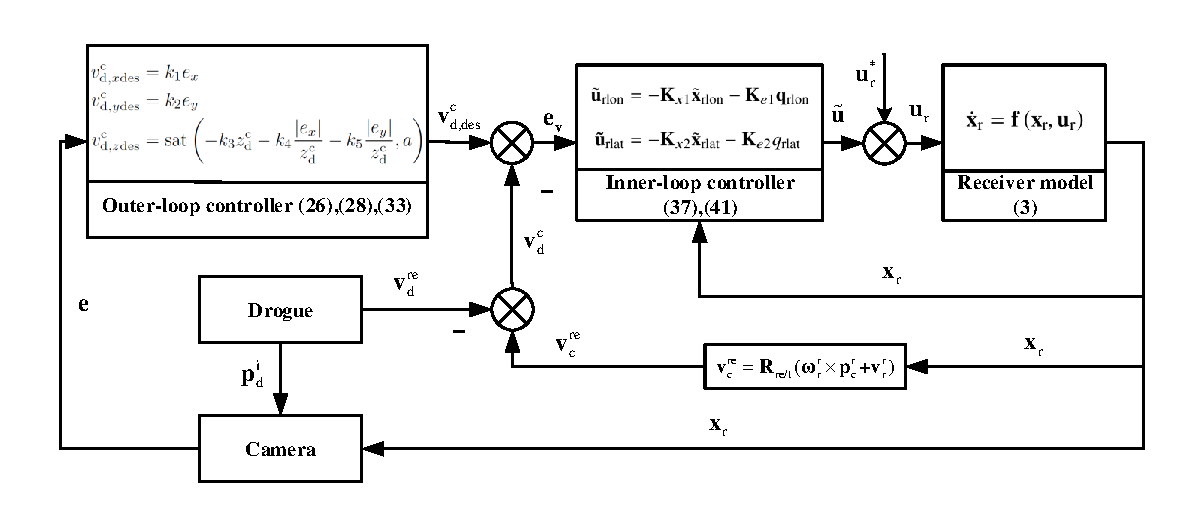
\includegraphics[width=0.9\textwidth]{Figures/Figs_Ch11/fig4.pdf}
	\caption{The closed-loop structure based on the designed IBVS controller.} \label{fig4}
\end{figure*} 



\section{Simulation and Verification}
In this section, various disturbances such as aerodynamic disturbance, tanker vortex disturbance, bow wave effect, and pose estimation errors are considered in the simulation to prove the validity of the designed controller.
\subsection{Simulation environment}
A high-fidelity simulation platform with a 3D virtual-reality visual display is built based on MATLAB/SIMULINK to simulate PDR docking. The basic information about this simulation platform can be referred to Refs. \cite{DAI2016448,7738351}. In this paper, the previous controller used in Refs. \cite{DAI2016448} is changed to the proposed IBVS
controller.


\subsection{Simulation results}
Different disturbances are set in the simulation environment to illustrate the performance of the designed IBVS controller. Besides, pose estimation errors are considered when making a comparison between IBVS and PBVS.


\subsubsection{Simulations under Aerodynamic Disturbance}   

The controller parameters of the outer-loop visual servo controller are set to the values in Table \ref{tab1}. At first, different intensities of the atmospheric disturbance are added. The intensity of the atmospheric disturbance is negatively correlated with the probability of the turbulence intensity being exceeded. In general, the intensity of the atmospheric disturbance of level \uppercase\expandafter{\romannumeral1} means that the probability of the turbulence intensity being exceeded is ${10^{ - 1}}$ and the maximum velocity of atmospheric disturbance is about $3$ feet per second. The level \uppercase\expandafter{\romannumeral2} means that the probability of the turbulence intensity being exceeded is ${10^{ - 2}}$ and the maximum velocity of atmospheric disturbance is about $5$ feet per second.
\begin{table}[h]
	\caption{Parameters of the outer-loop controller}
	\label{tab:Parameters of the outer loop}
	\centering
	\begin{tabular}{|l|c|c|c|c|c|c|}\hline
		Parameters&$ k_{1} $&$ k_{2} $&$ k_{3} $&$ k_{4} $&$ k_{5} $\\\hline
		Values&1&3&0.5&3&1\\\hline
	\end{tabular}\label{tab1}
\end{table} 

In Fig. \ref{fig5}, the intensity of aerodynamic disturbance is set at level \uppercase\expandafter{\romannumeral1} while the intensity of aerodynamic disturbance is set at level \uppercase\expandafter{\romannumeral2} in Fig. \ref{fig6}. It can be found that although the receiver's movement trajectory fluctuates with the increase of the wind disturbance intensity, the success of docking is ensured meanwhile the trajectory is relatively smooth due to the effect of the PI controller. Then, a bow wave effect is added in Fig. \ref{fig7} in which the controller parameters of the outer-loop visual servo controller are adjusted to the values in Table \ref{tab2}. Noteworthy, although the image tracking error fluctuates at the beginning, it can still guarantee the success of docking.	
\begin{table}[h]
	\caption{Parameters of the outer-loop controller under the bow wave effect and Level I aerodynamic disturbances}
	\label{tab:Parameters of the outer loop under the bow wave effect}
	\centering
	\begin{tabular}{|l|c|c|c|c|c|c|}\hline
		Parameters&$ k_{1} $&$ k_{2} $&$ k_{3} $&$ k_{4} $&$ k_{5} $\\\hline
		Values&1.6&5&0.5&3&1\\\hline
	\end{tabular}\label{tab2}
\end{table}

\begin{figure}[htbp]
	\centerline{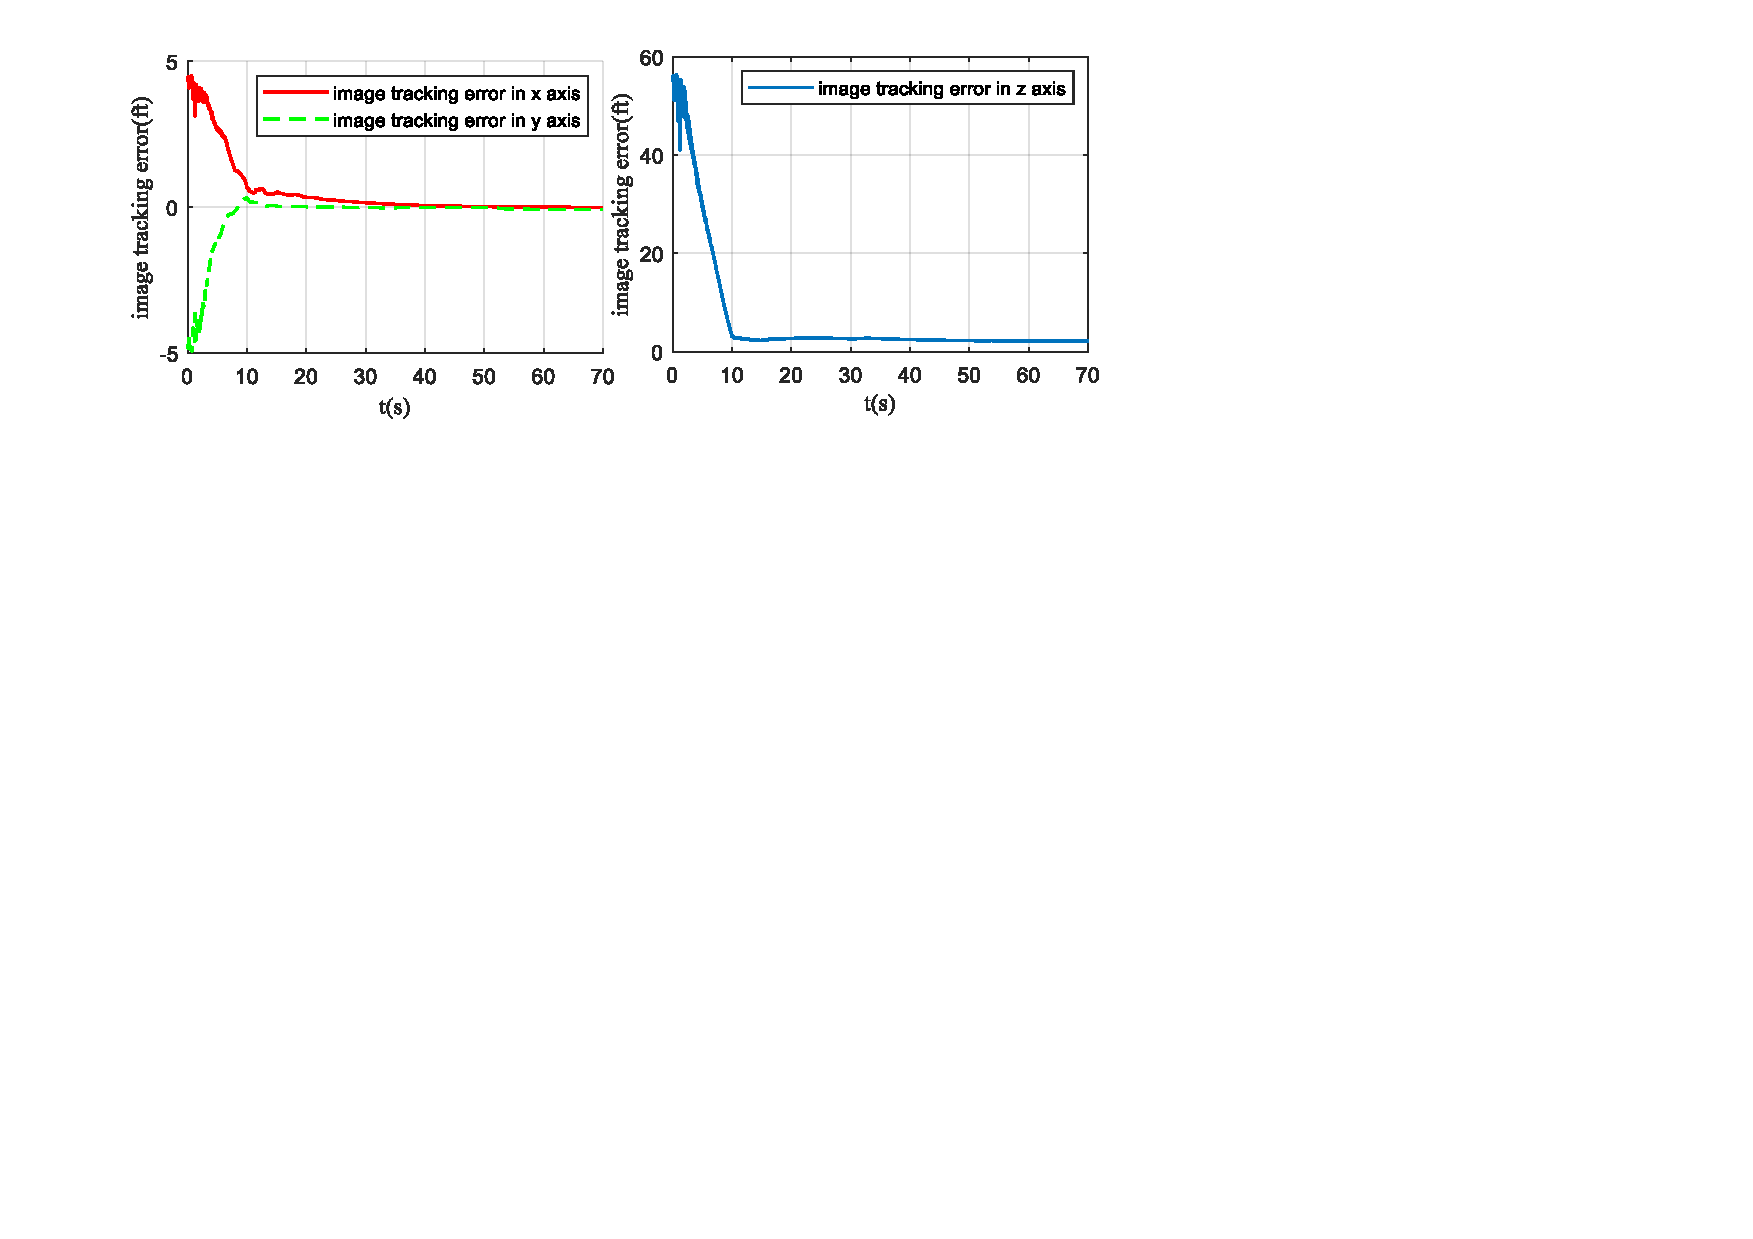
\includegraphics[width=.5\textwidth]{Figures/Figs_Ch11/fig5.pdf}}
	\caption{Image tracking error under different aerodynamic disturbances (Level I)}\label{fig5}
\end{figure}
\begin{figure}[htbp]
	\centerline{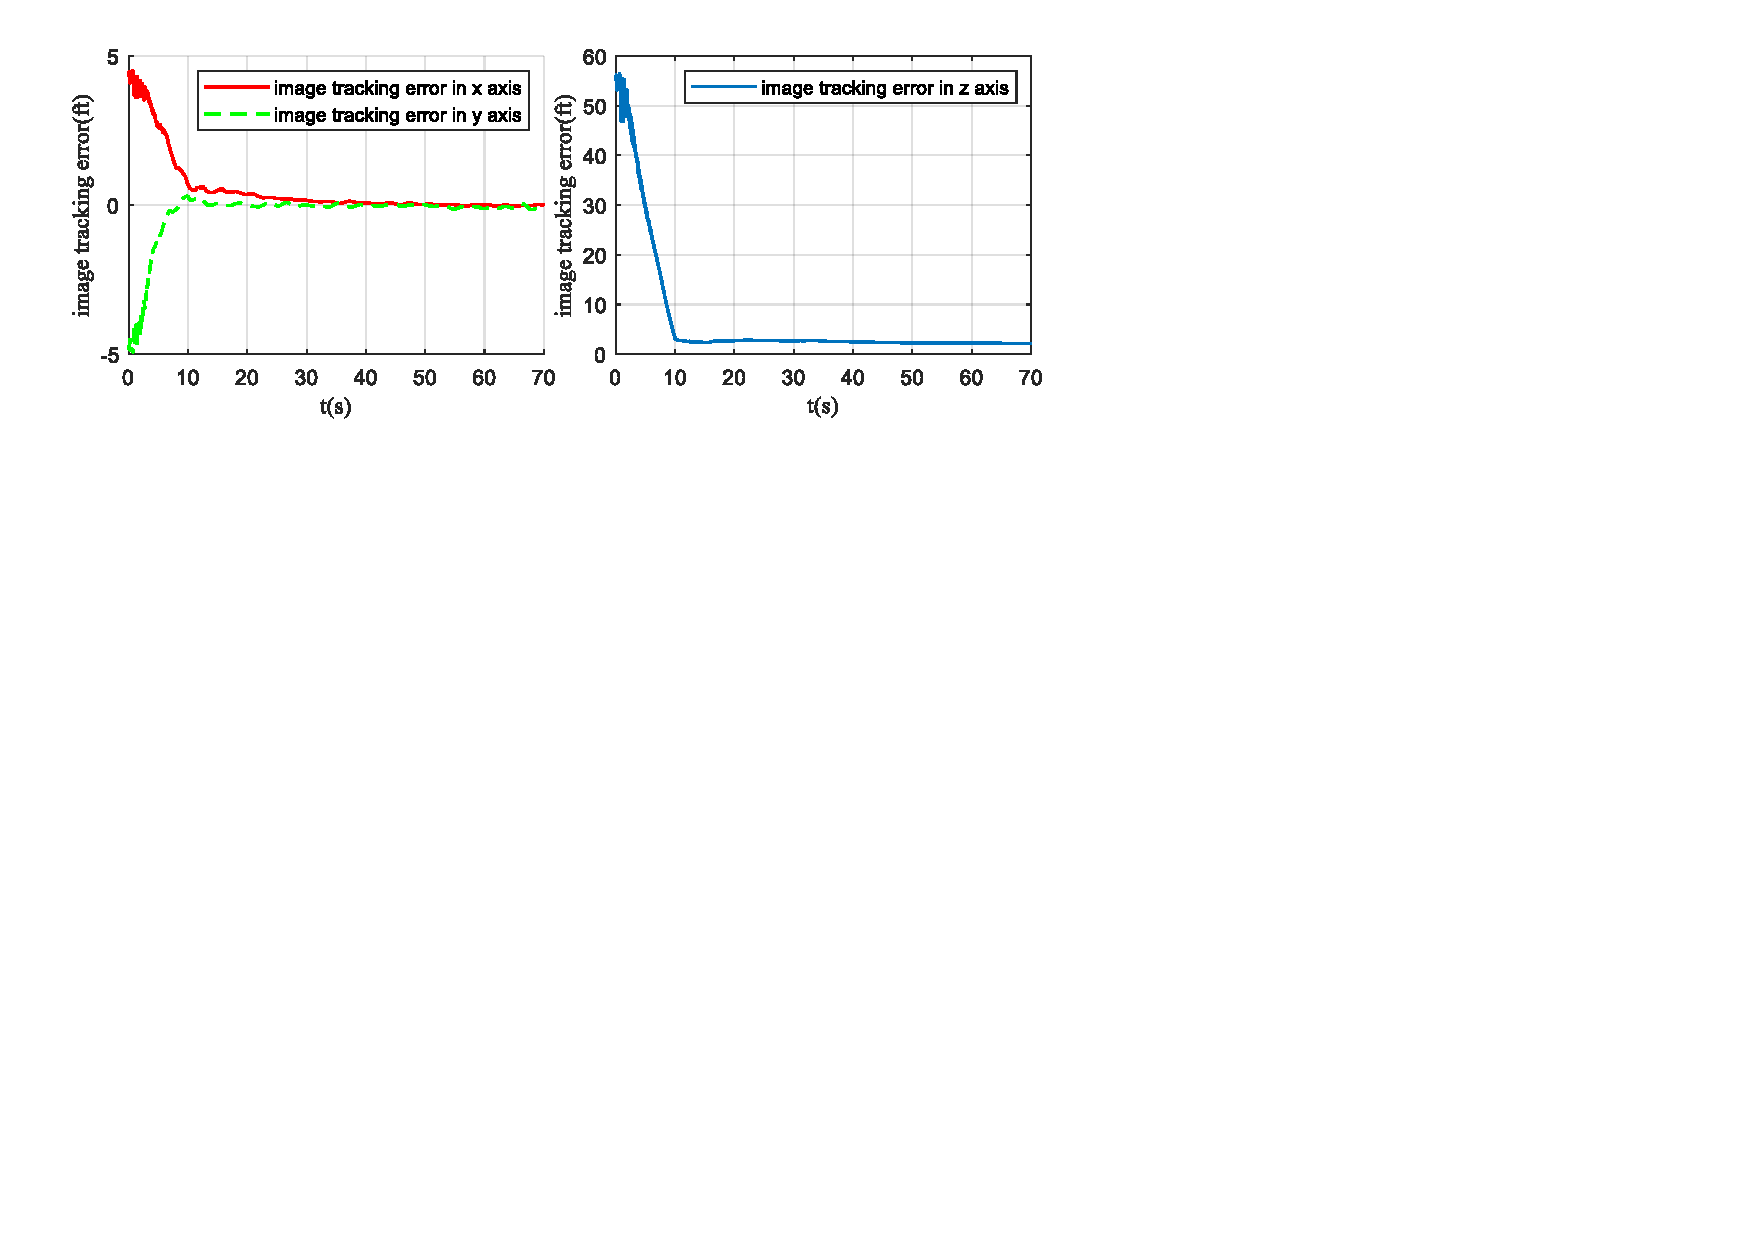
\includegraphics[width=.5\textwidth]{Figures/Figs_Ch11/fig6.pdf}}
	\caption{Image tracking error under different aerodynamic disturbances (Level II)}\label{fig6}
\end{figure}

\begin{figure}[htbp]
	\centerline{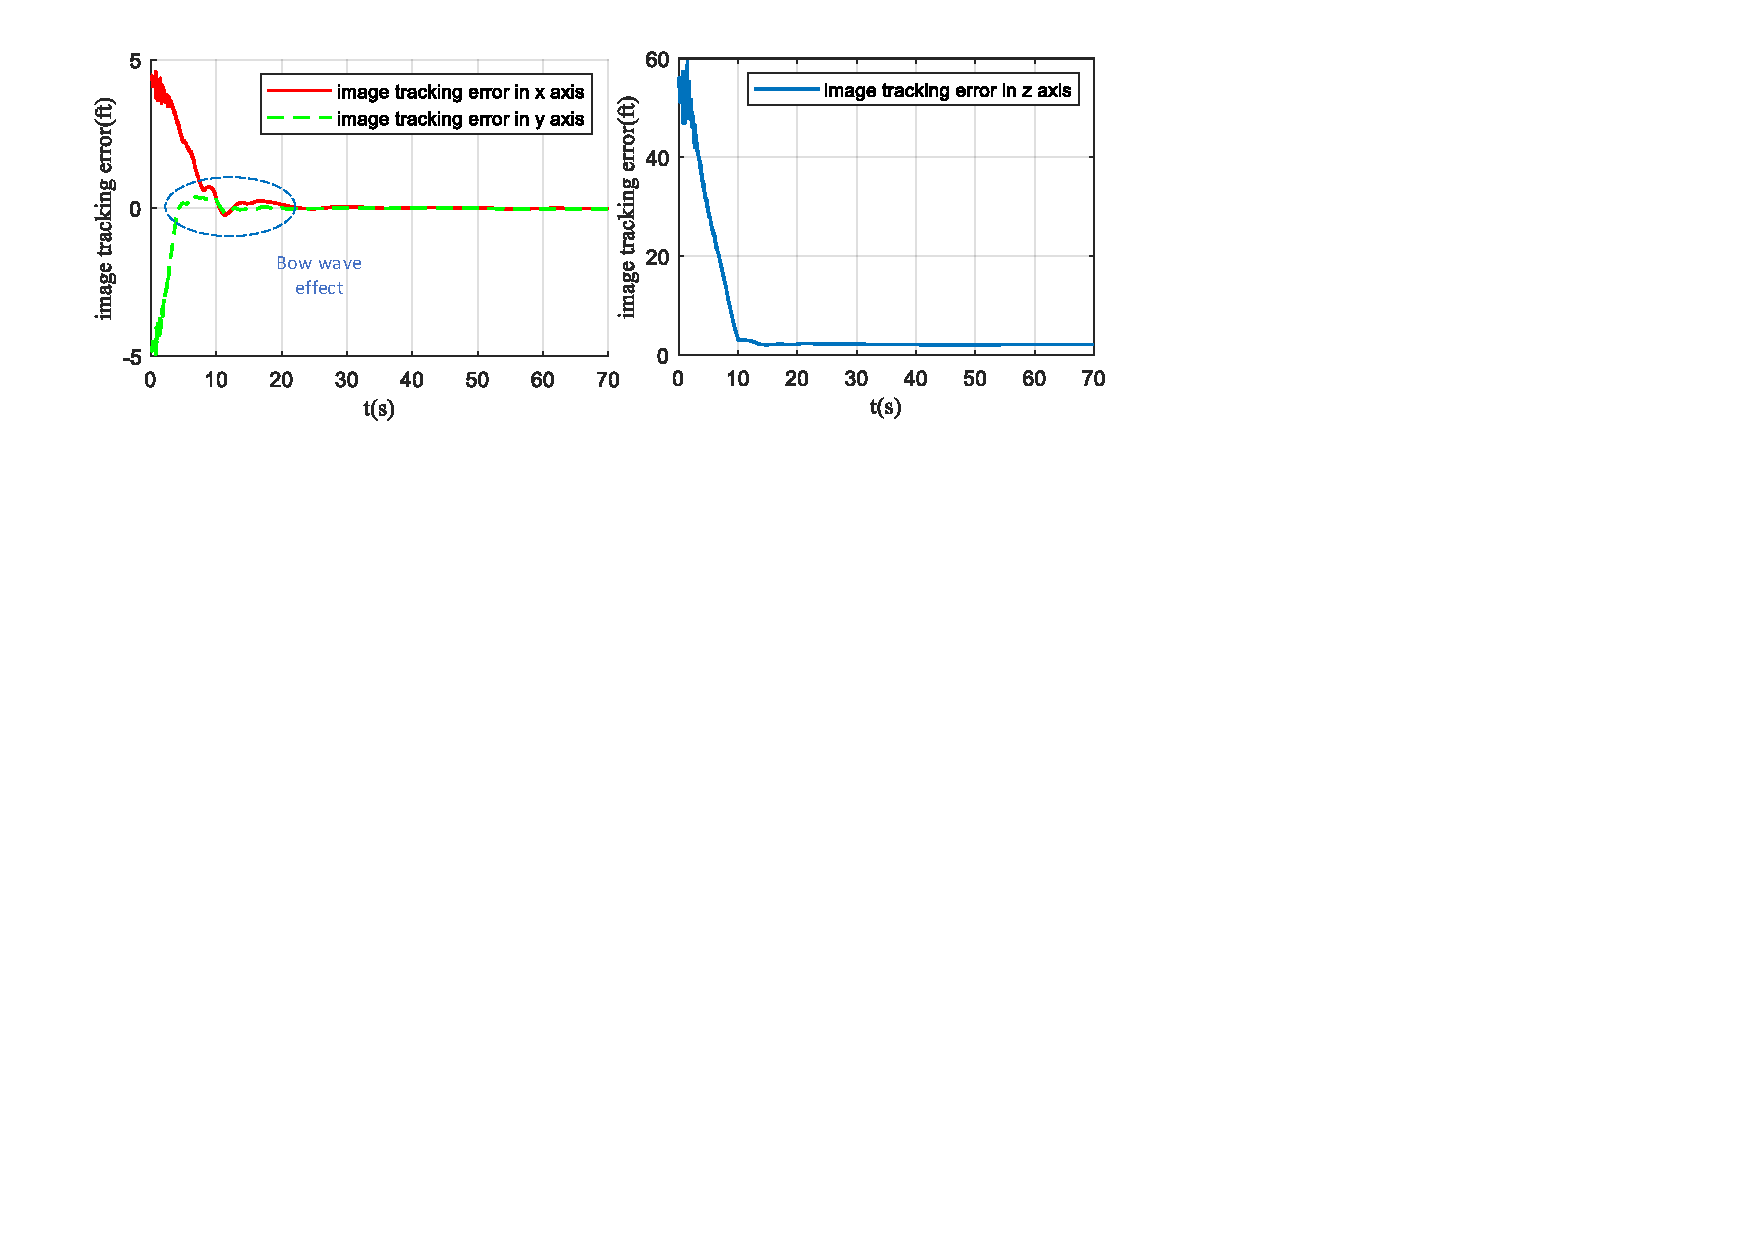
\includegraphics[width=.5\textwidth]{Figures/Figs_Ch11/fig7.pdf}}
	\caption{Image tracking error under bow wave effect and Level I aerodynamic disturbances}\label{fig7}
\end{figure}


\subsubsection{Simulations under Position Measurement Error}

Consider that the pose estimation error affects the docking control in two aspects: the camera installation position does not change, but the distance measurement may be inaccurate, or the distance measurement is precise,
but the actual position of the camera deviates from the original installation position. In order to simulate the situation that there are pose estimation errors during the PDR docking, $ \Delta \mathbf{p} _{\rm{c}}^{\rm{r}} = \left[ {\begin{array}{*{20}{c}}
	1&0&-0.5
	\end{array}} \right]
^{\rm{T}} $  is added to both IBVS and PBVS controllers, and the corresponding simulation results are shown in Fig. \ref{fig8}. It can be observed that the IBVS controller can perform successful docking while the PBVS cannot. 
\begin{figure}[htbp]
	\centerline{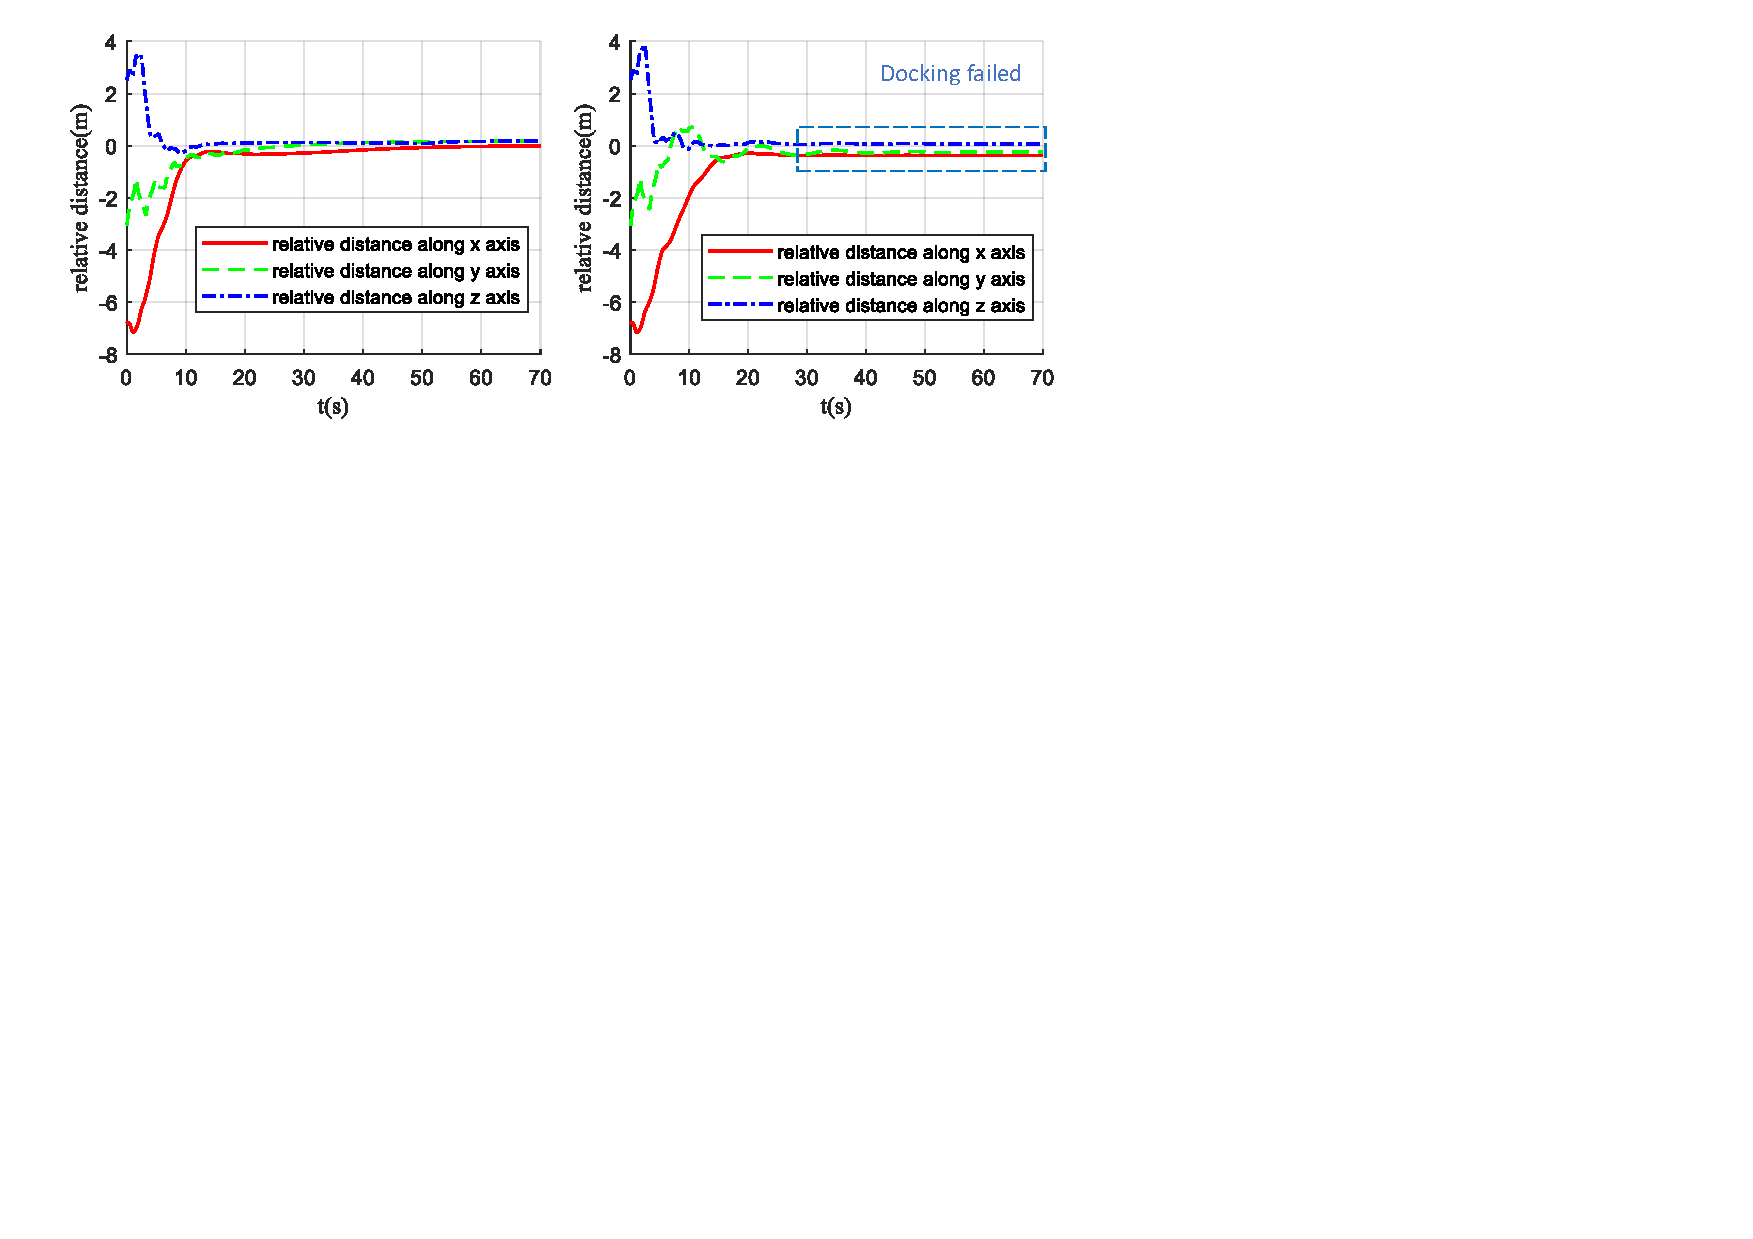
\includegraphics[width=.5\textwidth]{Figures/Figs_Ch11/fig8.pdf}}
	\caption{Image tracking error under position measurement error}\label{fig8}
\end{figure}

In order to better evaluate the docking performance and reliability of the proposed IBVS controller in the presence of pose estimation errors, a simple Monte Carlo simulation is also carried out. Position errors  $ \Delta \mathbf{p} _{\rm{c}}^{\rm{r}}= \left[ \Delta \mathbf{p} _{\rm{c,x}}^{\rm{r}}, \Delta \mathbf{p} _{\rm{c,y}}^{\rm{r}}, \Delta \mathbf{p} _{\rm{c,z}}^{\rm{r}} \right]^{\rm{T}} $used in the Monte Carlo simulations are listed in Table \ref{tab3}.

\begin{table}[h]
	\caption{Position errors used in the Monte Carlo
		simulations}
	\centering
	\begin{tabular}{|c|c|c|c|c|c|c|}\hline
		Pos. error&Nom. value&Max.&Min.&Distribution type\\\hline
		$\Delta \mathbf{p} _{\rm{c,x}}^{\rm{r}}$&0&1&-1&Uniform\\\hline
		$\Delta \mathbf{p} _{\rm{c,y}}^{\rm{r}}$&0&1&-1&Uniform\\\hline
		$\Delta \mathbf{p} _{\rm{c,z}}^{\rm{r}}$&0&1&-1&Uniform\\\hline
	\end{tabular}\label{tab3}
\end{table}

From the Monte Carlo simulations, the final docking success rate (DSR) can be obtained as shown in Table \ref{tab4}. It can be seen that IBVS control can achieve a 100\% docking success rate under light atmospheric turbulence, while the PBVS control can achieve a 70\% docking success rate under the same situation. When there exists strong atmospheric turbulence, the docking success rate of the IBVS and PBVS control all get worse, but the DSR of the IBVS control is still higher than the DSR of the PBVS control. Thus, it can be concluded that the IBVS control outperforms the PBVS control in the presence of position errors. Besides, it can be seen that the atmospheric turbulence intensity has a significant effect on the docking success.  
\begin{table}[h]
	\caption{Docking success rate of IBVS and PBVS control in the presence of position errors and turbulence disturbances}
	\centering
	\begin{tabular}{|c|c|c|c|c|c|c|}\hline
		\diagbox{{Controller}}{{DSR}}&  light tur. & strong tur. \\\hline
		IBVS&100\%&40\%\\\hline
		PBVS&70\%&10\%\\\hline
	\end{tabular}\label{tab4}
\end{table}


\subsubsection{Discussion}


For the visual servo control, as long as high-precision image information can be obtained, the calculated 3D relative position may be inaccurate due to the camera installation error, calibration error, and/or 3D object modeling error. In the simulation, the PBVS takes the 3D relative position as the outer-loop feedback. A PI controller can make the feedback error zero. However, there exists a position measurement error, and so the docking finally fails. On the contrary, the proposed IBVS takes the relative 2D image error as the outer-loop feedback. Errors existing in the inner loop are taken as constant disturbances. Besides, the depth error does not determine the docking success that much like the 2D image error. As a result, the IBVS controller is more robust against measurement errors than the PBVS controller. 



\section{Chapter Summary}
This paper proposes an IBVS model for the probe-and-drogue refueling and an IBVS docking control method. Concretely, the IBVS control for the outer loop and the LQR control for the inner loop are designed to improve the robustness of the docking control. Simulations show that the proposed IBVS controller has enough robustness, which can achieve a successful docking in the precence of complex disturbances and pose estimation errors. Here, the control surfaces and the throttle are control inputs of the system. However, the low-level controller has always been finished or cannot be changed for safety in practice. Therefore, further research, based on an existing low-level controller,  where the velocity is adopted as the control input is worth studying. Besides, the velocity controller often aims at the receiver's position control. However, the velocity controller for PDR docking needs to control the position of the probe tip, which is related to the receiver's attitude. This is full of challenges.